% !TeX encoding = UTF-8
% !TeX program = xelatex
% !TeX spellcheck = fr
\documentclass[10pt,a4paper]{report}
\usepackage[informatique]{styles/preambule_college}
\usepackage{styles/preambule_personnalisation}



% ----------------------------------------------------------------------
% Compilation chapitre par chapitre
% ----------------------------------------------------------------------
%\includeonly{choix_extensions_ch10_bibliographies}
%\includeonly{choix_extensions_ch08_maths}
%\includeonly{choix_extensions_ch03_pages}
%\includeonly{choix_extensions_ch07_tableaux}



% ----------------------------------------------------------------------
% Packages et configurations spéciales pour le fichier avec les exemples
% LaTeX
% ----------------------------------------------------------------------
\usepackage{lipsum}					% Génère un texte sans signification (Lorem ipsum)
\usepackage[final]{showexpl}		% Permet d'afficher un code LaTeX en parallèle de son résultat
%									% N.B. ce package appelle le package listings pour la présentation du code
\AtBeginDocument{%
	\renewcommand*\lstlistlistingname{Examples}
	\renewcommand*\lstlistingname{Example}
}
\declaretheoremstyle[notefont=\bfseries,parent=chapter,shaded={bgcolor=yellow}]{exempleStyle}
\declaretheorem[style=exempleStyle,name=Définition]{boxedDefinition}





% ----------------------------------------------------------------------
% Début du document
% ----------------------------------------------------------------------
\begin{document}

	\chapterFormat % Active le format personnalisé pour les titres de chapitres

	% !TeX encoding = UTF-8
% !TeX root = choix_extensions.tex
% ----------------------------------------------------------------------------------------------------------------
% Page de titre
% ----------------------------------------------------------------------------------------------------------------

\begin{titlepage}
	\begin{center}
		\vspace*{3cm}
		
		\Huge{
			Choix d'extensions \LaTeX
			
			pour le collège
		}

		\vspace*{3cm}
		
		\Huge{
			Trucs \& astuces
		}
		
		\vspace{12cm}
		
		\small{
			Samuel Vannay
			
			14.09.2022
			
			\ccLogo \ccAttribution \ccNonCommercialEU \ccShareAlike
		}
	\end{center}

\end{titlepage}
 




% ----------------------------------------------------------------------------------------------------------------
% Table des matières avec numérotation des pages en chiffres romains
% ----------------------------------------------------------------------------------------------------------------

\pagenumbering{roman}
%\dominitoc[n]

\tableofcontents
%\faketableofcontents   % A décommenter si on ne veut pas de table des matières principale, mais uniquement les tables par chapitre

\vfill

Cette {\oe}uvre est mise à disposition selon selon les termes de la \href{http://creativecommons.org/licenses/by-nc-sa/3.0/ch/deed.fr}{licence Creative Commons Attribution - Pas d'Utilisation Commerciale - Partage dans les Mêmes Conditions 3.0 Suisse (CC BY-NC-SA 3.0 CH)}
	\pagenumbering{arabic}
	% !TeX encoding = UTF-8
% !TeX root = choix_extensions.tex
\chapter{Prise en main}






\section{Introduction}

Ce document décrit comment mettre en place un environnement de travail \LaTeX \ fonctionnel basé sur la distribution \TeX \ Live, l'éditeur TeXstudio et les fichiers de style \incmd{preambule_college.sty} et \newline
\incmd{preambule_personnalisation.sty}. Il regroupe des trucs et astuces qui m'ont pris du temps à trouver et à mettre au point. En cas de remarque : \href{mailto:samuel.vannay@edu.vs.ch}{samuel.vannay@edu.vs.ch}.



\subsection{Pour les impatients}


\subsubsection{Pour commencer sans distribution}

Pas besoin d'installer quoi que ce soit pour commencer à apprendre les bases de \LaTeX. Il suffit d'essayer en ligne sur
\begin{center}
	\href{https://www.learnlatex.org/fr/}{Learn\LaTeX.org}.
\end{center}

Pas besoin non plus d'installer quoi que ce soit pour commencer à travailler. Il suffit de créer un compte sur
\begin{center}
	\href{https://www.overleaf.com/}{Overleaf}.
\end{center}


\subsubsection{Installer et configurer}

Installations requises :
\begin{enumerate}
	\item \TeX \ Live avec toutes ses collections (cf. captures dans la fiche \emph{Mise en place de son environnement de travail});
	\item TeXstudio;
	\item optionnellement, pour ceux qui doivent mettre en forme du code informatique, Anaconda pour avoir Python avec la librairie Pygments.
\end{enumerate}

Configurations à faire à la main :
\begin{enumerate}
	\item Dans TeXstudio (cf. captures \ref{sec:installationTl}) :
		\begin{itemize}
			\item au besoin rajouter les options de compilation \incmd{-shell-escape} et \incmd{-8bit} aux compilateurs;
			\item choisir \XeLaTeX \ comme compilateur par défaut;
			\item choisir \incmd{biber} comme outil de bibliographie par défaut.
		\end{itemize}
	\item Copier les fichiers du répertoire \incmd{cwl} dans :
		\begin{itemize}
			\item $\sim$\incmd{/.config/texstudio/completion/user} sous Linux et Mac OS;
			\item généralement dans \lstinline!%APPDATA%\texstudio\completion\user! sous Windows.
		\end{itemize}
\end{enumerate}


\subsubsection{Utilisation}

Dans TeXstudio :

\begin{enumerate}[a.]
	\item Placer le répertoire \incmd{styles} au même endroit que le document principal.
	\item Personnaliser \incmd{style/preambule_personalisation.sty}, notamment les mots-clés pdf.
	\item Dans le document principal appeler \inlatex{\usepackage[informatique]{styles/preambule_college}} avec ou sans l'option informatique, et \inlatex{\usepackage{styles/preambule_personnalisation}}
		\attention L'option \incmd{informatique} nécessite qu'une distribution Python avec la librairie Pygments soit installée.
	\item Utiliser les exemples de ce document pour les mises en page particulières.
	\item Compiler avec \XeLaTeX \ de la dernière version de \TeX \ Live.
\end{enumerate}





\newpage






\section{Distribution \LaTeX}
\label{sec:distributionLaTeX}







\subsection{Choix de la distribution}

La distribution la plus portable et qui contient uniquement des extensions libres est
\begin{center}
	\href{http://www.tug.org/texlive/}{\TeX \ Live}.
\end{center}

Pour plus de détails, consultez la \href{http://tug.org/texlive/doc/texlive-fr/texlive-fr.pdf}{documentation} officielle\footnote{Pour des variantes, voir cet \href{http://tex.stackexchange.com/questions/239199/latex-distributions-what-are-their-main-differences}{article}.}.



\subsection{Lancer l'installation}

\begin{description}
	\item[\textcolor{red}{pour Linux}] ~\\
		Soit une version est déjà présente, soit elle est disponible dans les dépôts. Mais il vaut la peine d'envisager de désinstaller la version présente et d'installer la version originale à la place. \\
		\textbf{Prérequis : } \incmd{perl-tk} et \incmd{whish} \quad (si nécessaire : \incmd{sudo apt install perl-tk whish} ou équivalent).
		\begin{itemize}
			\item En ligne
				\begin{itemize}
					\item Télécharger et décompresser \href{http://mirror.ctan.org/systems/texlive/tlnet/install-tl-unx.tar.gz}{install-tl-unx.tar.gz}.
					\item Exécuter \incmd{sudo ./install-tl gui} dans le répertoire décompressé.
				\end{itemize}
			\item Hors ligne
				\begin{itemize}
					\item Télécharger le \href{http://mirror.ctan.org/systems/texlive/Images/}{fichier ISO};
					\item Copie ce fichier sur l'ordinateur hors ligne;
					\item l'ouvrir et exécuter \incmd{sudo ./install-tl gui} dans le répertoire de base.
				\end{itemize}
		\end{itemize}
	\item[\textcolor{red}{pour Mac}] ~\\
		Télécharger et installer \href{http://www.tug.org/mactex}{MacTeX}.
	\item[\textcolor{red}{pour Windows}] ~\\
		\attention Sous Windows, l'installation peut être bien longue\dots
		\begin{itemize}
			\item En ligne \\
				Télécharger et exécuter \href{http://mirror.ctan.org/systems/texlive/tlnet/install-tl-windows.exe}{install-tl-windows.exe}.
			\item Hors ligne
				\begin{itemize}
					\item Télécharger le \href{http://mirror.ctan.org/systems/texlive/Images/}{fichier ISO};
					\item Transférer ce fichier sur l'ordinateur hors ligne
					\item L'ouvrir\footnote{Sous certaines versions de Windows, il faut éventuellement installer un utilitaire pour lire le fichier .iso, par exemple \href{http://wincdemu.sysprogs.org/}{winCDEmu}.}, clic droit sur \incmd{install-tl-advanced.exe} qui s'y trouve et \newline \incmd{Exécuter en tant qu'administrateur}.
				\end{itemize}
		\end{itemize}
\end{description}



\subsection{Options d'installation}

Une fois le menu d'installation affiché (pareille pour toutes les plates-formes), on choisit ce qu'on veut. Ici : tout sauf les langues dont on ne va pas se servir (voir les captures d'écran \ref{sec:installationTl}).



\subsection{Utilisation de \TeX \ Live}

Facile : on n'y touche pas !

\remarque*{
	Au besoin, on peut ajouter et retirer des packages avec l'utilitaire \incmd{tlmgr} (voir \ref{sec:majTl}) fourni avec la distribution. Sous Mac OS, cet utilitaire s'appelle \incmd{Tex Live Utility}. \\
	On peut aussi installer la nouvelle version de TeX Live qui sort chaque année au printemps%\dots
}





\section{Éditeur}
\label{sec:Editeur}



\subsection{Choix de l'éditeur}

Le meilleur éditeur libre, offrant exactement la même interface pour Linux, Mac OS et Windows, complet et personnalisable est 
\begin{center}
	\href{http://www.texstudio.org/}{TeXstudio}.
\end{center}

Sa prise en main est rapide\footnote{Pour des alternatives, consultez cet \href{https://en.wikipedia.org/wiki/Comparison_of_TeX_editors}{article} Wikipédia.}.



\subsection{Installation}

\href{http://www.texstudio.org/}{Télécharger} la dernière version et exécuter l'installateur \emph{après} avoir installé \TeX \ Live. De cette manière, il s'intègre à \TeX \ Live tout seul comme un grand.



\subsection{Configuration}

Dès que TeXstudio est installé, il faut faire quelques configurations dans le menu
\begin{center}
	\incmd{Options} \textrightarrow \ \incmd{Configurer TeXstudio...} \quad (ou équivalent sous Mac OS)
\end{center}
Voir les captures de \ref{sec:configTeXstudio}.


\subsubsection{Activer l'appel des scripts externes}

Pour autoriser TeXstudio à appeler des scripts externes comme Pygments, il faut ajouter une option dans la commande qui est passée au compilateur dans la boîte de dialogue \incmd{Configurer TeXstudio}, partie \incmd{Compilations}, rajouter dans les lignes \incmd{PDFLaTeX}, \incmd{XeLaTeX} et \incmd{LuaLaTeX} l'option
\begin{center}
	\incmd{ -shell-escape } \quad (espace avant et espace après)
\end{center}


\subsubsection{Accepter les caractères sur 8 bits}

Pour permettre à \TeX \ Live de gérer sans souci les caractères sur 8 bits, rajouter l'option à vos compilateurs.
\begin{center}
	\incmd{ -8bit } \quad (espace avant et espace après, pas de "s")
\end{center} 


\subsubsection{Choix du compilateur par défaut}

Le compilateur est le logiciel fourni dans \TeX \ Live qui transforme le code \LaTeX \ en document pdf. Il en existe plusieurs : \LaTeX, PDF\LaTeX, Lua\LaTeX \dots

Ici le choix est d'utiliser
\begin{center}
	\XeLaTeX \quad (prononcer Zee Lay Tech).
\end{center}

Ce compilateur prend en charge les caractères Unicode (notamment l'encodage UTF-8 qui est devenu le standard sur tous les ordinateurs) et permet d'utiliser les polices de caractères vectorielles de son ordinateur.

\begin{center}
	\incmd{Configurer TeXstudio} \textrightarrow \ \incmd{Production} \textrightarrow \  \incmd{XeLaTeX} comme compilateur par défaut (voir \ref{sec:configTeXstudio}).
\end{center}


\subsubsection{Réglage de l'auto-complétion}
	
Le fichier \incmd{preambule_college.sty} contient de nombreuses nouvelles commandes. Il est possible de les déclarer à TeXstudio de manière à ce qu'elles apparaissent dans l'auto-complétion et l'analyseur syntaxique. Pour cela, il faut créer un fichier \incmd{cwl} (voir le fichier \incmd{preambule_college.cwl} fourni) et le placer dans le répertoire :
\begin{itemize}
	\item $\sim$\incmd{/.config/texstudio/completion/user} sous Linux et Mac OS;
	\item généralement dans \lstinline!%APPDATA%\texstudio\completion\user! sous Windows.
\end{itemize}

Ensuite, TeXstudio peut charger ce fichier \incmd{.cwl} automatiquement, mais pour s'assurer que c'est chaque fois le cas, il vaut mieux l'activer manuellement dans :
\begin{center}
	Menu \incmd{Options} \textrightarrow \ \incmd{Configurer TeXstudio} \textrightarrow \ Onglet \incmd{Complétion}
\end{center}



%\subsubsection{Mise en place du modèle de polycopié}
%
%Il est possible de faire des modèles de document et de les déclarer à TeXstudio. Un modèle de polycopié a été préparé pour faciliter la création de document multi-fichiers. Pour l'activer, il faut copier les fichiers \newline \incmd{template_polycop.zip}, \incmd{template_polycop.json} et \incmd{template_polycop.png} dans le répertoire :
%\begin{itemize}
%	\item $\sim$\incmd{/.config/texstudio/template/user} sous Linux et Mac OS;
%	\item généralement dans \lstinline!%APPDATA%\texstudio\template\user! sous Windows.
%\end{itemize}






\section{Produire un code maintenable}

Avec \LaTeX \ on sépare le contenu de la forme. Le principe de base en \LaTeX \ est donc le suivant :

\begin{center}
	\begin{boxedminipage}{.75\textwidth}
		\textcolor{red}{\textbf{Utilisez \emph{systématiquement} des raccourcis (les créer au besoin) qui décrivent le contenu et non la mise en forme.}}
		
		\textcolor{red}{Le fichier \incmd{preambule_college.sty} contient une quantité de raccourcis de ce type qu'il faut utiliser systématiquement. Ce document les présente en détail.}
	\end{boxedminipage}
\end{center}

Cela permet de modifier ensuite globalement l'apparence d'un document sans avoir à en modifier le contenu. 

\exemple*{	
	Dans les définitions mathématiques, on veut réserver une mise en forme spéciale pour les mots faisant l'objet de la définition. Certains préfèrent les mettre en italique, d'autres en gras. Dans ce cas, on procède de la manière suivante :
	\begin{enumerate}
		\item Convenir d'une balise commune, ici \mintinline{latex}{\emphdef}.
		\item Définir cette balise dans un fichier \incmd{.sty}. Ici, \incmd{preambule_college.sty} contient : \newline
		\mintinline{latex}{\newcommand{\emphdef}[1]{\emph{\#1}}} \footnote{\mintinline{latex}{\newcommand} débute la création d'une nouvelle commande, \incmd{[1]} spécifie qu'on va donner une série de mots en paramètre de la commande. La suite indique de mettre en italique les mots passés en paramètres.}.
		\item Utiliser systématiquement cette balise pour les définitions dans le fichier \incmd{.tex}.
		\item Pour adapter l'apparence des mots définis à ce qu'on veut, il suffit de changer la description de \mintinline{latex}{\emphdef}, ce qui est d'ailleurs le cas dans le fichier \incmd{preambule_personnalisation.sty} : \newline
		\mintinline{latex}{\renewcommand{\emphdef}[1]{\textbf{#1}}} \newline
		Ceci écrase l'ancienne définition et fait afficher les mots définis en gras.
	\end{enumerate}
}




\section{Où placer ses fichiers .sty}



\subsection{Pour éviter tout problème}

Quand on copie le répertoire exemple, tout est prêt pour travailler sans mauvaise surprise : le sous-répertoire \incmd{style} contient les fichiers \incmd{preambule_college.sty} et \incmd{preambule_personalisation.sty}.

De cette manière, on peut personnaliser son document (hiérarchie de la numérotation, mots-clés pour les méta-informations pdf, licences d'utilisation\dots) et si les fichiers de style viennent à évoluer indépendamment de ce document particulier, on a la garantie de pouvoir toujours le compiler avec l'ancienne version des styles.



\subsection{Pour une configuration centralisée}

Il est possible (et déconseillé) de placer les \incmd{.sty} dans un seul endroit d'où ils seront accessibles pour tous les documents. Il y en a qui ont essayé : ils ont eu des problèmes\dots

Les répertoires centraux sont les suivants :
\begin{itemize}
	\item Linux \incmd{~/texmf/tex/latex/local/}
	\item Mac OS X \incmd{<user name>/Library/texmf/tex/latex/local/}
	\item Windows \Verb!C:\Users\<user name>\texmf\tex\latex\local\!
\end{itemize}

Après avoir placé les fichiers dans ces répertoires, il faut encore signaler leur présence à \LaTeX \ soit avec \TeX Live Manager (\incmd{tlmgr}), soit à la ligne de commande (\incmd{texhash}, voire \incmd{mktexlsr}). Voir la  \href{http://tug.org/texlive/doc/texlive-fr/texlive-fr.pdf}{documentation} de \TeX \ Live pour plus d'informations.





\section{Captures d'écran}
\label{sec:captures}



\subsection{Configurer l'installation de \TeX \ Live}
\label{sec:installationTl}

Ces captures ont été faites durant l'installation d'une version \TeX \ Live 2021 sous Linux. C'est quasiment pareil pour Windows et entièrement différent pour Mac\dots

\begin{figure}[H]
	\centering
	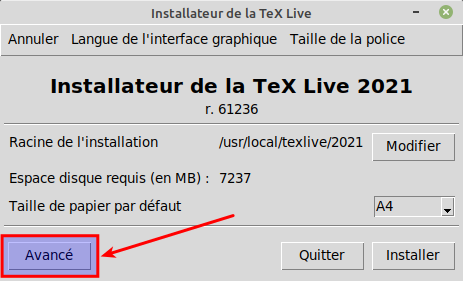
\includegraphics[width=6cm]{captures/install_TL_01.png}
	\caption{Mode avancé}
	\label{fig:captureTLInstall01}
\end{figure}

\begin{figure}[H]
	\centering
	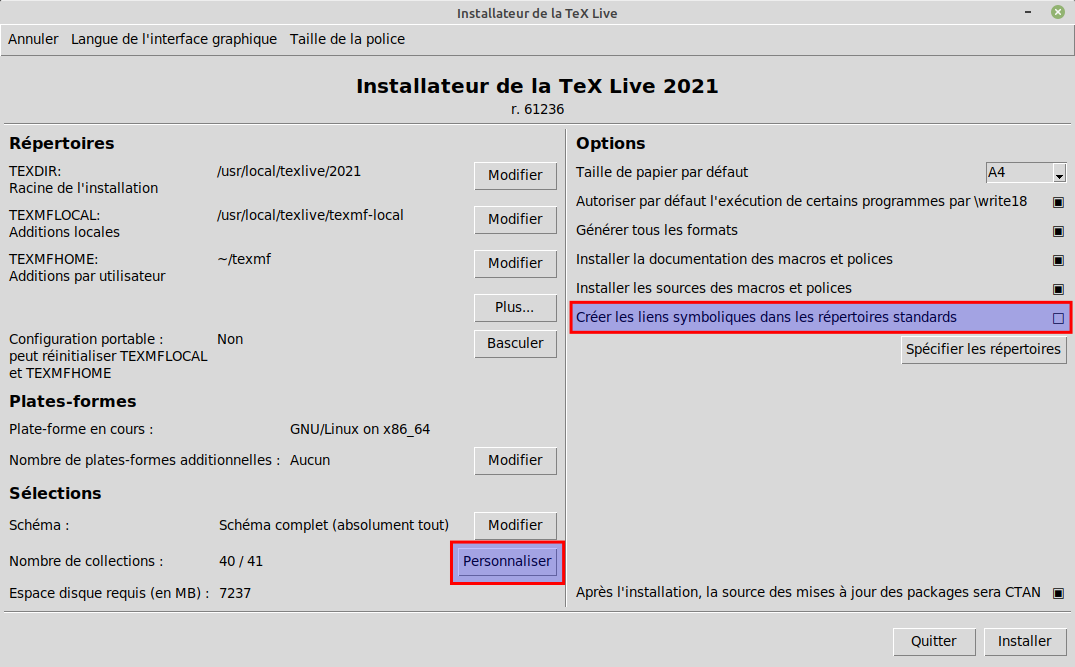
\includegraphics[width=15cm]{captures/install_TL_02.png}
	\caption{Faire créer les liens et choisir les collections}
	\label{fig:captureTLInstall02}
\end{figure}

\begin{figure}[H]
	\centering
	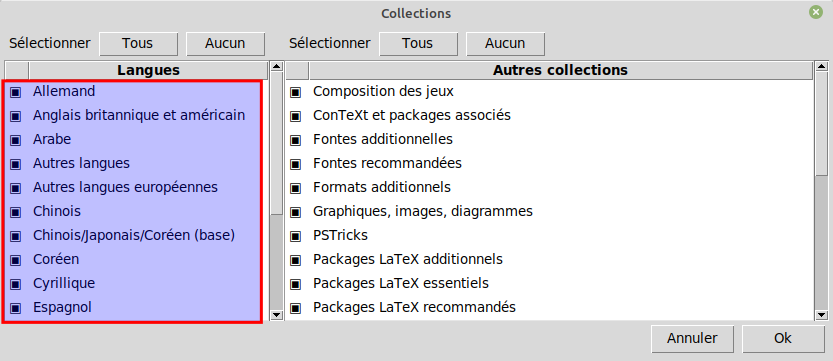
\includegraphics[width=10cm]{captures/install_TL_03.png}
	\caption{Ne garder que le français}
	\label{fig:captureTLInstall03}
\end{figure}



\subsection{Mettre \TeX \ Live à jour}
\label{sec:majTl}


\subsubsection{Linux et Windows}

\begin{figure}[H]
	\centering
	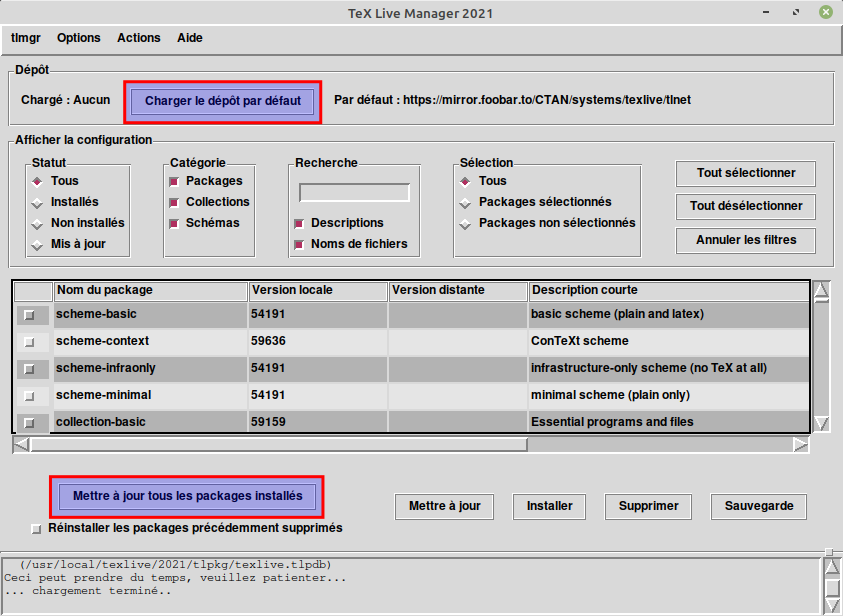
\includegraphics[width=\linewidth]{captures/TL_manager_2021.png}
	\caption{Activer les dépôts et lancer la mise à jour}
	\label{fig:captureTLInstall01}
\end{figure}


\subsection{Configurer TeXstudio}
\label{sec:configTeXstudio}

\begin{figure}[H]
	\centering
	\includegraphics[width=\linewidth]{captures/configurer_TeXstudio_compilations}
	\caption{Configuration de TeXstudio - Compilations}
	\label{fig:captureConfigTeXstudioCompilations}
\end{figure}

\begin{figure}[H]
	\centering
	\includegraphics[width=\linewidth]{captures/configurer_TeXstudio_production}
	\caption{Configuration de TeXstudio - Production}
	\label{fig:captureConfigTeXstudioProduction}
\end{figure}





\subsection{Fichiers fournis}

\begin{enumerate}
	\item \incmd{choix_extensions.pdf} ce document.
	\item \incmd{cwl/} répertoire pour déclarer les raccourcis à TeXstudio.
	\item \incmd{sources/} les sources pour créer ce document.
	\item \incmd{styles/}
	\begin{enumerate}[a.]
		\item \incmd{styles/preambule_college.sty} \\
		choix organisé et commenté d'extensions et de raccourcis utiles pour la mise en forme de documents généraux, mathématiques et informatiques. L'option \inlatex{informatique} permet d'activer les packages et raccourcis pour mettre en page du code informatique. \\
		\attention L'option \inlatex{informatique} requière l'installation de Python et de sa librairie Pygments au préalable. Le plus simple est d'installer \href{https://www.anaconda.com/products/individual}{Anaconda}.
		\item \incmd{styles/preambule_personalisation.sty} \\
		réglages qui sont propres à chaque nouveau document. Ce fichier {\color{red}{\textbf{doit être adapté pour chaque nouveau document.}}}
	\end{enumerate}
\end{enumerate}





	% !TeX encoding = UTF-8
% !TeX root = choix_extensions.tex
\chapter[Fichiers et compilation]{Gestion des fichiers et compilation}
\label{ch:compilation}






\section{Fichiers multiples et magic comments}

Lorsqu'un document a été séparé en multiples fichiers (un fichier principal et un fichier par chapitre), on travaille surtout dans les fichiers des chapitres. Malheureusement, ils ne peuvent pas être compilés tels quels (ils n'ont pas de préambule ni d'environnement \mintinline{latex}{document}). En principe, TeXstudio est assez malin pour appeler le compilateur sur le fichier principal, mais pas toujours. Pour assurer le coup, il y a deux possibilités : 
\begin{enumerate}
	\item Placer dans chaque fichier contenant un chapitre le magic comment\footnote{Les magic comments sont des commentaires spéciaux qui servent à configurer TeXstudio. Ils se placent tout en début de fichier et commencent par \texttt{\% !TeX}. Ces paramètres surchargent les paramètres de TeXstudio et permettent donc un paramétrage document par document.} : \newline
		\lstinline|% !TeX root = doc_principal.tex| où "doc\_principal.tex est le nom du document maître.
	\item Fixer à la main le fichier principal. Afficher le fichier en question puis aller dans le menu \newline
		\incmd{Options} \textrightarrow \incmd{Définir le document en cours comme "Document maître"}. \newline
		\textbf{Attention :} si on ouvre un nouveau document, le compilateur ne s'en occupe pas, il continue à compiler le document maître. Tant qu'on n'a pas réalisé l'erreur, on peut s'arracher pas mal de cheveux\dots
\end{enumerate}

\remarque*{
	Tant qu'à faire, il y a d'autres magic comments qui peuvent nous éviter des soucis :
	\begin{enumerate}
		\item Dans le document maître : \mintinline{latex}{program = xelatex}
		\item Dans chaque fichier : \mintinline{latex}{encoding = UTF-8}
		\item Dans chaque fichier : \mintinline{latex}{TeX spellcheck = fr}
	\end{enumerate}
	Ces magic comments sont disponibles dans le menu \incmd{LaTeX} \textrightarrow \incmd{Ajouter des commentaires magiques...} et dans les menus déroulants \incmd{Langue} et \incmd{Codage d entrée} tout en bas à droite de la fenêtre TeXstudio.
}






\section{PDF d'un seul chapitre}
\label{sec:multidoc}

Il faut isoler chaque chapitre dans un fichier et les inclure dans le document principal à l'aide de la commande \mintinline{latex}{\include{nom_fichier}}.

Par exemple, supposons que le fichier \incmd{document_principal.tex} contienne \mintinline{latex}{\include{ch01}}, \mintinline{latex}{\include{ch02}} et \mintinline{latex}{\include{ch03}}. Pour obtenir un pdf contenant seulement le chapitre 3, tout en respectant toutes les numérotations (chapitres, pages\dots), il faut :
\begin{enumerate}
	\item compiler une fois le document avec tous les chapitres (pour mettre à jour les fichiers auxiliaires);
	\item dans le préambule, ajouter (ou décommenter) la commande \mintinline{latex}{\includonly{ch03}};
	\item compiler à nouveau le document.
\end{enumerate}

Voir l'exemple suivant.





\newpage





\begin{minipage}{.55\linewidth}
	\begin{minted}{latex}
\documentclass{article}
\includeonly{ch03}
\begin{document}
\include{ch01}
\include{ch02}
\include{ch03}\end{document}

% Remarquez les numéros de titre et de page
	\end{minted}
\end{minipage}
\hfill
\begin{boxedminipage}{.38\linewidth}
	\centering
	
\includegraphics[scale=.5]{images/choix_extensions_exemple_principal}
\end{boxedminipage}





\section[Versions d'un document]{Différentes versions d'un même document}

Pour faire différentes versions d'un même document, utiliser la \emphdef{compilation conditionnelle} avec l'extension \mintinline{latex}{optional}.

Par exemple, pour une compilation destinée uniquement aux élèves, on appelle l'extension \mintinline{latex}{optional.sty} avec l'option \mintinline{latex}{eleves} dans le préambule : \mintinline{latex}{\usepackage[eleves]{optional}}. Puis, dans le fichier, on place les parties uniquement destinées aux élèves dans les deuxièmes accolades d'une commande \mintinline{latex}{\opt{eleves}{}}.

\begin{minipage}{.6\linewidth}
	\begin{minted}{latex}
\documentclass[twoside]{report}
\usepackage[eleves]{optional}

\begin{document}
  \opt{eleves}{cf. formulaires p. 92}} :
  \[
    1+\frac{1}{1!}+\frac{1}{2!}+\dots = \opt{prof}{e}
   \]
\end{document}
	\end{minted}
\end{minipage}
\hfill
\begin{boxedminipage}{.35\linewidth}
	cf. formulaires p. 92 :
	\[
		1+\frac{1}{1!}+\frac{1}{2!}+\dots =
	\]
\end{boxedminipage}

Le même fichier peut contenir une variante pour les professeurs. Dans ce cas, il faut appeler \mintinline{latex}{optional} avec \newline \mintinline{latex}{usepackage[prof]{optional}} dans le préambule et placer le code destiné aux professeurs dans le deuxième argument d'une commande \mintinline{latex}{\opt{prof}{}}.

\begin{minipage}{.6\linewidth}
	\begin{minted}{latex}
\documentclass[twoside]{report}
  \usepackage[prof]{optional}

  \begin{document}
  \opt{eleves}{cf. formulaires p. 92}} :
  \[
    1+\frac{1}{1!}+\frac{1}{2!}+\dots = \opt{prof}{e}
  \]
\end{document}
	\end{minted}
\end{minipage}
\hfill
\begin{boxedminipage}{.35\linewidth}
	\[
		1+\frac{1}{1!}+\frac{1}{2!}+\dots = e
	\]
\end{boxedminipage}

\remarque*{
	Cette pratique est dangereuse pour vos informations : il est facile de se tromper et de transmettre une version du document aux mauvaises personnes. Pour éviter ceci, il est recommandé de créer une copie du document principal pour chaque version, ayant chacune son option pour \mintinline{latex}{\uespackage[...]{optional}}.
}



\section{Insérer une licence Creative Commons}

Pour commencer, il faut choisir sa licence sous \url{http://creativecommons.org/choose/}, par exemple by-nc-as (Creative Commons Attribution - Pas d'Utilisation Commerciale - Partage dans les Mêmes Conditions).

Sur le site de Creative Commons, récupérer la phrase à faire figurer dans le document; ici : "Cette {\oe}uvre est mise à disposition selon les termes de la \href{http://creativecommons.org/licenses/by-nc-sa/3.0/ch/deed.fr}{licence Creative Commons Attribution - Pas d'Utilisation Commerciale - Partage dans les Mêmes Conditions 3.0 Suisse (CC BY-NC-SA 3.0 CH)}".

Eventuellement, récupérer l'image correspondant à la licence, ici : 
\includegraphics[height=2ex]{images/licence_CC_BY_NC_SA}, ou utiliser les commandes de l'extension \href{http://mirror.ctan.org/fonts/ccicons/ccicons.pdf}{\mintinline{latex}{ccicons}} :
\begin{LTXexample}[pos=o,width=.15]
\ccLogo, \ccAttribution, \ccNonCommercial, \ccShareAlike
\end{LTXexample}

Dans le fichier \mintinline{latex}{styles_document.sty}, dans la première section du document, il faut copier la phrase et l'URL de la licence dans la première partie du document, par exemple :	
\begin{minted}{latex}
\hypersetup{
  pdftitle={Choix de l'extension LaTeX pour le collège},
  pdfsubject={Trucs & astuces pour gagner en efficacité et en portabilité},
  pdfkeywords={LaTeX} {Collège} {college} {trucs} {astuces} {efficacité} {portabilité}
    {package}{exemple},
  pdfauthor={Samuel Vannay},
  %Pour insérer une licence Creative Commons (machine readable) dans le fichier pdf
  pdfcopyright={Cette oeuvre est mise à disposition selon les termes de la Licence 
    Creative Commons Attribution - Pas d'Utilisation Commerciale - Partage dans les
    Mêmes Conditions 3.0 Suisse (CC BY-NC-SA 3.0 CH)},
  pdflicenseurl={http://creativecommons.org/licenses/by-nc-sa/3.0/ch}
}
\end{minted}

De cette manière, le fichier pdf contient toutes les informations, lisibles par n'importe qui, mais aussi lisibles par les moteurs de recherches.
	% !TeX encoding = UTF-8
% !TeX root = choix_extensions.tex
\chapter{Mise en page et titres}
\label{ch:miseEnPage}





\section{Choix de la fonte}



\subsection{Quelques informations}
\begin{itemize}
	\item \XeLaTeX \ est notamment conçu pour pouvoir utiliser les fontes Open Type (\incmd{.otf}), True Type (\incmd{.ttf}) et Apple Advance Typogaphy (\incmd{.aat}) du système sur lequel on travaille. Étonnamment, si \XeLaTeX \ voit les fontes du système, il ne voit pas forcément celles de \TeX \ Live sans configuration supplémentaire\dots
	
	\item Dans \LaTeX, les fontes ont quatre paramètres :
	\begin{enumerate}
		\item la famille de fontes : avec empattement, sans empattement, à chasse fixe, mathématique;
		\item la série : la quantité de graisse;
		\item la forme : droite, penchée, italique, en petite capitale;
		\item le corps : la taille de la fonte.
	\end{enumerate}
	\item Les bonnes fontes sont livrées avec une italique redessinée (qui n'est pas une simple version penchée), avec une petite capitale redessinée (qui n'est pas une capitale d'un autre corps), avec une italique grasse et avec toute une série de ligatures.
\end{itemize}



\subsection{Fonte du système}

On peut regarder le nom d'une fonte dans un autre logiciel, p. ex. avec LibreOffice, ou avec le gestionnaire de fonte. Puis on choisit cette fonte avec l'une des commandes : 

\begin{itemize}
	\item \mintinline{latex}{\setmainfont{nom de la fonte}} ou souvent \mintinline{latex}{\setromanfont} pour la fonte romaine de base;
	\item \mintinline{latex}{\setsansfont{nom de la fonte}} pour la fonte sans empattement;
	\item \mintinline{latex}{\setmonofont{nom de la fonte}} pour la fonte à chasse fixe;
	\item \mintinline{latex}{\setmathfont{nom de la fonte}} pour la fonte mathématique.
\end{itemize}

\remarque*{
	Ces commandes sont chatouilleuses : il faut faire attention aux espaces, aux accents, à la casse.
}



\subsection{Fonte \TeX \ Live}
\label{sec:fonteTeXLive}


\subsubsection{Appeler directement les fontes \TeX \ Live}
\TeX \ Live dispose de nombreuses fontes qui se trouvent dans le répertoire de la distribution (p. ex. sous Linux dans \incmd{/usr/local/texlive/2015/texmf-dist/fonts}). On peut accéder aux fontes True Type ou Open Type s'y trouvant en spécifiant leur nom de fichier. Il faut alors spécifier les fichiers correspondant aux différentes séries et formes disponibles (gras, italique, petite capitale, gras italique) si elles existent.

\begin{minted}{latex}
\setmainfont{texgyrepagella-regular.otf}[
  BoldFont=texgyrepagella-bold.otf,
  ItalicFont=texgyrepagella-italic.otf,
  BoldItalicFont=texgyrepagella-bolditalic.otf
]
\setmathfont{texgyrepagella-math.otf}
\end{minted}


\subsubsection{Voir toutes les fontes système disponibles sous Linux}

Pour obtenir la liste des fontes disponibles sous Linux : \lstinline!fc-list :outline -f "%{family}\n" | sort -u!.


\subsubsection{Rendre les fontes de \TeX \ Live visibles par le système}

\attention ceci va faire déferler des hordes de fontes \LaTeX \ Open Type et True Type sur le système. Cette opération dépend du système. Version proposée par ce \href{http://texnique.fr/osqa/questions/115/listes-des-fontes-disponibles}{forum} :
\begin{description}
	\item[Linux] copier le fichier \incmd{/usr/local/texlive/2015/texmf-var/fonts/conf/texlive-fontconfig.conf}, supprimer la ligne se terminant par \incmd{fonts/type1</dir>} et le placer :
	\begin{enumerate}
		\item en tant qu'utilisateur standard : en \incmd{~/.fonts.conf} (si ce fichier existe déjà, il ne faut pas l’écraser, mais fusionner les deux en recopiant les lignes commençant par \incmd{<dir>} du fichier de \TeX \ Live entre \incmd{<fontconfig>} et \incmd{</fontconfig>} dans le fichier existant) puis on lance la commande \incmd{fc-cache};
		\item (si on désire installer ces fontes pour tous les utilisateurs) en tant qu’administrateur : en \newline
		\incmd{/etc/fonts/conf.d/09-texlive.conf} puis on lance la commande \incmd{fc-cache -s}.
	\end{enumerate}
	\item[Mac OS X] ouvrir l’application Livre des fontes puis le menu Fichier → Nouvelle bibliothèque pour créer une nouvelle bibliothèque nommée par exemple \incmd{TeX Live}, qu’on sélectionne ensuite. On ouvre alors le menu \incmd{Fichier} \textrightarrow \incmd{Ajouter des fontes} et, dans la boîte qui apparaît, on utilise le raccourci \incmd{Maj + Cmd + G} pour aller dans le dossier \incmd{/usr/local/texlive/2015/texmf-dist/fonts} où on sélectionne les répertoires opentype et truetype avant de valider.
	\item[Windows] Il n’y a rien à faire, l’installateur \TeX \ Live s’est occupé de tout.
\end{description}



\subsection{Fonte mathématique}

Il n'y a que peu de fontes Open Type Math complètes et qui se comportent gentiment et poliment avec les accents : Latin Modern Math, XITS Math, STIX Math, Asana Math, TeX Gyre Pagella Math\footnote{Il y a aussi d'autres fontes de TeX Gyre qui ont une version Math : Bonum Math, Schola Math, Termes Math (à essayer et bien vérifier avant d'adopter).}.

Pour changer de fonte mathématique, il faut encore faire attention à la cohérence entre les nombres utilisés dans les zones mathématiques et les zones gérées par \incmd{siunitx}. Par exemple, si on veut une fonte Linux Libertine pour le texte et une fonte Pagella Math pour les maths :


\subsubsection{Variante A : les fontes \TeX \ Live sont connues du système}
\begin{minted}{latex}
%
% Pour la fonte de texte
%
\defaultfontfeatures{Scale=MatchLowercase,Ligatures=TeX,Mapping=tex−text}
\setmainfont{Linux Libertine}
%
% Pour la fonte mathématique et les nombres du texte
%
\unimathsetup{math-style=ISO}
\setmathfont{TeX Gyre Pagella Math}[Scale=MatchLowercase]
\newfontfamily\pagellaM[Numbers=Lining]{TeX Gyre Pagella Math}
\sisetup{mode = text,number-text-rm = \pagellaM}
\end{minted}

Avec ça, les nombres dans les parties mathématiques et dans les parties gérées par \incmd{siunitx} sont en Pagella. Les nombres dans les parties texte restent en Libertine\footnote{Ca n'a pas l'air franchement évident de faire en sorte que tous les nombres soient les mêmes. En cas de besoin, mieux vaut utiliser \inlatex{\num{1234}} pour mettre 1234 en fonte mathématique.}.


\subsubsection{Variante B : les fontes \TeX \ Live ne sont pas vues par le système}
\begin{minted}{latex}
%
% Pour la fonte de texte
%
\defaultfontfeatures{Scale=MatchLowercase,Ligatures=TeX,Mapping=tex−text}
%\setmainfont{Linux Libertine}
%\setmonofont{Linux Libertine Mono}[Scale=MatchLowercase]
%\setsansfont{Linux Biolinum}[Scale=MatchLowercase]
\setmainfont{LinLibertine_R.otf}[
		BoldFont=LinLibertine_RB.otf,
		ItalicFont=LinLibertine_RI.otf,
		BoldItalicFont=LinLibertine_RBI.otf	
	]
\setmonofont{LinLibertine_M.otf}[Scale=MatchLowercase]
\setsansfont{LinBiolinum_R.otf}[Scale=MatchLowercase]
%
% Pour la fonte mathématique
%
\unimathsetup{math-style=ISO}
\setmathfont{texgyrepagella-math.otf}[Scale=MatchLowercase]
\newfontfamily\pagellaM[Numbers=Lining]{texgyrepagella-math.otf}
\sisetup{mode = text,number-text-rm = \pagellaM}
\end{minted}


\subsection{Fontes supplémentaires}

Question de base : est-ce vraiment une si bonne idée ? Si oui\dots


\subsubsection{Fontes non libres de \TeX \ Live}

Pour installer les fontes non libres de \TeX \ Live \url{http://www.tug.org/fonts/getnonfreefonts/}.


\subsubsection{Quelques ressources}

\begin{itemize}
	\item Exemples :
		\href{http://www.math.ucsd.edu/~msharpe/ffsamples.pdf}{ffsamples.pdf},
		\href{http://www.tug.org/fonts/special-s.pdf}{\TeX \ font sampler} (voir les informations à la fin du document);
	\item Identifier des fontes :
		\href{http://www.identifont.com/similar.html}{Identifon};
	\item Liste des fontes de \TeX Live
		\href{https://www.ctan.org/topic/font-otf}{Open Type}
			\footnote{\label{foot:fontePackage} \attention il ne faut pas appeler l'extension correspondante, mais seulement la fonte en question, selon le mécanisme décrit dans \ref{sec:fonteTeXLive}.},
		\href{https://www.ctan.org/topic/font-ttf}{True Type}\footref{foot:fontePackage}, et
		\href{https://www.ctan.org/topic/font-maths}{mathématiques},
		\href{http://www.tug.dk/FontCatalogue/}{The \LaTeX \ Font Catalogue} (toutes les fontes);
	\item Fonderies et dépôts libres :
		\href{http://www.sil.org/resources/software_fonts}{SIL}, \href{http://www.gust.org.pl/projects/e-foundry/tex-gyre/}{TeX Gyre},
		\href{http://www.fontsquirrel.com}{Font Squirrel},
		\href{http://www.exljbris.com}{exljbris},
		\href{http://delubrum.org/}{Delubrum},
		\href{https://fontlibrary.org/}{Open Font Library},
		\href{http://fontsgeek.com}{fontsgeek.com},
		\href{http://www.dafont.com/fr/}{dafont.com};
	\item Fonderies commerciales :
		\href{http://www.linotype.com/fr/}{Linotype},
		\href{http://www.fontspring.com}{Fontspring},
		\href{http://www.adobe.com/products/type/fonts-by-adobe.html}{Adobe},
		\href{https://typekit.com}{Adobe Typekit}.
\end{itemize}





\section{Gestion des longueurs (length)}
\label{sec:gestionLongueurs}

Parfois, il est nécessaire d'afficher les valeurs numériques de longueurs pour les régler finement. Dans ce cas, l'extension \mintinline{latex}{\usepackage{printlen}} fournit la commande \mintinline{latex}{\printlength} :

\begin{LTXexample}[pos=o]
\printlength{\linewidth}
\end{LTXexample}
 





\section{Page de titre}

La page de titre s'obtient avec l'environnement \mintinline{latex}{\begin{titlepage}} :
	
\vspace{1em}
\begin{minipage}{.48\linewidth}
	\begin{minted}{latex}
\documentclass[twoside]{report}
\usepackage[a6paper]{geometry}
\usepackage{titlesec}
\usepackage[latin1]{inputenc}
\usepackage{ccicons}

\begin{document}
  \begin{titlepage}
    \vspace{5cm}
    \centerline{\Huge{Géométrie première}}
    \vspace{.3cm}
    \centerline{\LARGE Support de cours}
    \vspace{7cm}
    \centerline{Commission de géométrie}
    \centerline{Version 2011-2012}
    \centerline{
    \ccLogo \ccAttribution
    \ccNonCommercialEU \ccShareAlike
  }
  \end{titlepage}
\end{document}
	\end{minted}
\end{minipage}
\hfill
\begin{boxedminipage}{.4\linewidth}
	\centering
	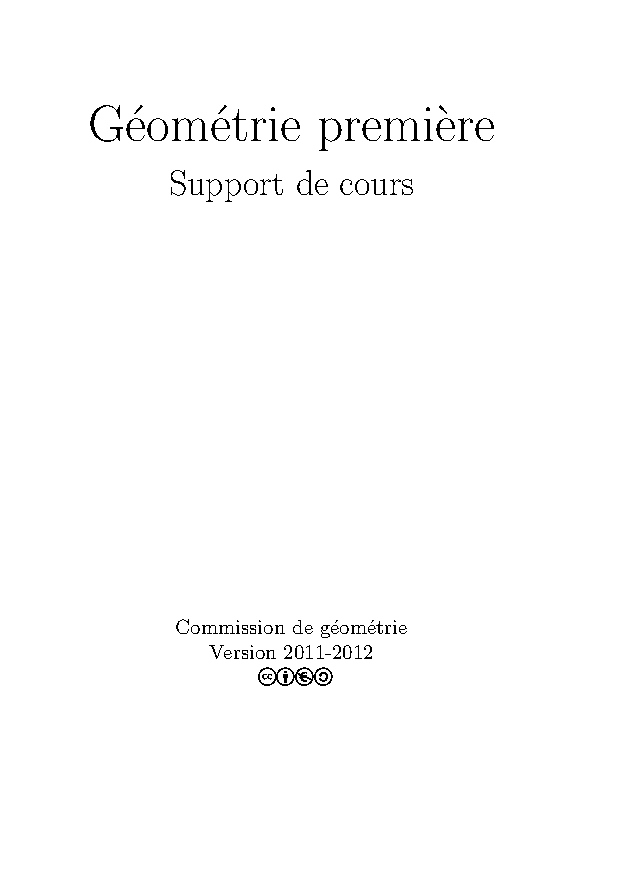
\includegraphics[scale=.5]{images/choix_extensions_exemple_titlePage}
\end{boxedminipage}
	
	
	
	

\section{Personnalisation des titres}



\subsection{Apparence des titres}

Les titres de chapitres, sections\dots \ peuvent être personnalisés grâce à l'extension \href{http://mirror.ctan.org/macros/latex/contrib/titlesec/titlesec.pdf}{titlesec}. Par exemple, les titres de chapitre de ce document sont définis dans \incmd{preambule_personalisation.sty} par le code suivant :

\begin{minted}{latex}
\titleformat{\chapter}[frame]        % frame pour avoir un cadre
    {\normalfont\small\scshape}      % Format du bandeau
    {\ Chapitre \thechapter\ }       % Texte du bandeau
    {.5cm}              % avec frame : esp. vertical autour du titre
    {\LARGE\bfseries\filcenter}[]    % avant la composition du titre

\titlespacing{\chapter} % régler l'espacement autour du titre de chapitre
    {0pt}   % à gauche
    {-1cm}  % avant
    {1cm}   % après
    [0pt]   % à droite
\end{minted}

Pour plus de souplesse, notamment pour pouvoir changer de style entre les chapitres normaux et ceux de l'annexe, ce code a été introduit dans une commande : \mintinline{latex}{\newcommand{\chapterFormat}{...}}. Cette commande est appelée dans le fichier principal de ce document (\mintinline{latex}{choix_extensions.tex}).



\subsection{Numérotation des titres}

Si on veut éviter que les titres de sections reprennent le numéro du chapitre en cours, il faut dé-commenter la ligne suivante dans \incmd{preambule_personalisation.sty} : \mintinline{latex}{\renewcommand{\thesection}{\arabic{section}}}. Il est aussi possible d'insérer cette commande en cours de document.





\newpage






\section{Interligne}

Pour régler l'interligne avec l'extension \href{http://ctan.org/pkg/setspace}{setspace} : en utilisant les commandes \mintinline{latex}{\singlespacing}, \mintinline{latex}{\onehalfspacing}, et \mintinline{latex}{\doublespacing}. Par exemple : 
\begin{LTXexample}[pos=o,width=.5]
\onehalfspacing
Donec in nisl. Fusce vitae est. Vivamus ante ante, mattis laoreet, posuere eget, congue vel, nunc. Fusce sem. Nam vel orci eu eros viverra luctus. Pellentesque sit amet augue. Nunc sit amet ipsum et lacus varius nonummy.
\end{LTXexample}

On obtient le même effet pour l'ensemble du document avec les options : \mintinline{latex}{singlespacing}, \mintinline{latex}{onehalfspacing} et \mintinline{latex}{doublespacing}. Par exemple avec \mintinline{latex}{\usepackage[onehalfspacing]{setspace}}.





\section{En-tête et pied de page personnalisés}

À faire avec l'extension \href{http://mirror.ctan.org/macros/latex/contrib/fancyhdr/fancyhdr.pdf}{fancyhdr}. Par exemple, \incmd{preambule_personnalisation.sty} du présent document contient :

\begin{minted}{latex}
\pagestyle{fancy}
\renewcommand{\chaptermark}[1]{\markboth{\thechapter. \ #1}{}}
\renewcommand{\sectionmark}[1]{\markright{\thesection\ #1}}
\fancyhf{}
\fancyhead[LO,RE]{\bfseries \rightmark}
\fancyhead[LE,RO]{\bfseries \leftmark}
\fancyfoot[C]{\thepage}
\fancypagestyle{plain}{
    \fancyhead{}
    \renewcommand{\headrulewidth}{0pt}
    \fancyfoot[C]{\thepage}
}
\setlength\headheight{15pt}
\end{minted}





\section{Table des matières par chapitre}

Avec l'extension \href{http://mirror.ctan.org/macros/latex/contrib/minitoc/minitoc-fr.pdf}{\mintinline{latex}{minitoc}}. Attention, actuellement, il est commenté dans le fichier \incmd{preambule_college.sty}. Sans cela, il interfère et génère une page vide à la fin du document\dots

\begin{itemize}
	\item Dans le préambule : placer \mintinline{latex}{\dominitoc[n]} et soit \mintinline{latex}{\tableofcontents}, soit \mintinline{latex}{\faketableofcontents} si on ne veut pas de table globale.
	\item Dans le document : insérer \mintinline{latex}{\minitoc} où l'on veut la table.
\end{itemize}

\begin{minipage}{.48\linewidth}
	\begin{minted}{latex}
\documentclass[a4paper,twoside]{report}
\usepackage{minitoc}
\dominitoc[n]
\faketableofcontents
\begin{document}
\chapter{Mon chapitre}
\section{Dans ce chapitre}
\minitoc
\section{Ma section 1}
\subsection{Ma section 1}
    bla bla
\section{Ma section 2}
    bla bla
\end{document}
	\end{minted}
\end{minipage}
\hfill
\begin{boxedminipage}{.4\linewidth}
	\centering
	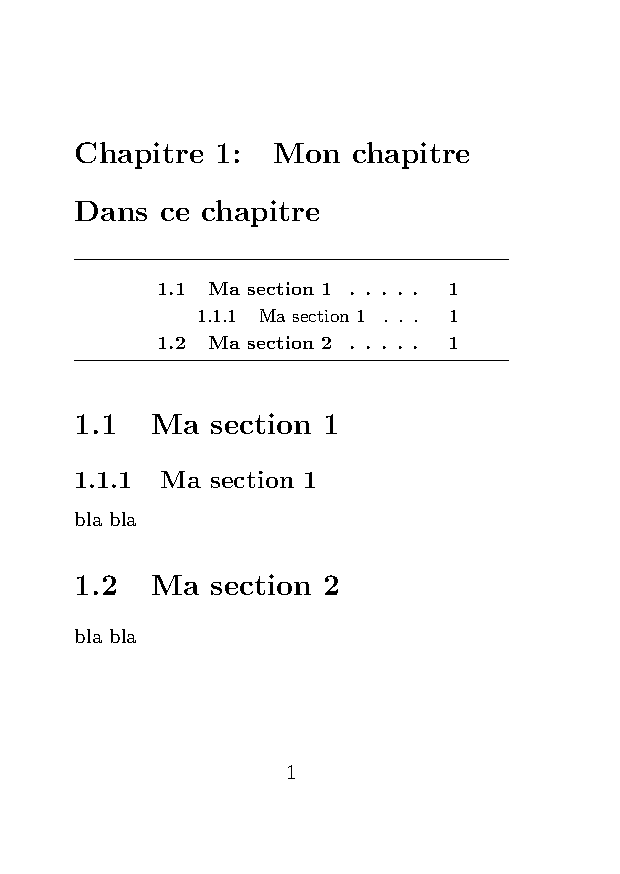
\includegraphics[scale=.5]{images/choix_extensions_exemple_minitoc}
\end{boxedminipage}





\section{Boîte autour d'une minipage}
Avec l'extension \href{http://mirror.ctan.org/macros/latex/contrib/boxedminipage/boxedminipage.pdf}{boxedminipage} (documentation plutôt sommaire !) :
\begin{LTXexample}[pos=o,width=.4]
\begin{boxedminipage}[t]{3cm}
    Voyez le brick géant que j'examine près du wharf.
\end{boxedminipage}
\begin{boxedminipage}[t]{3cm}
    Quel beau bateau\dots
\end{boxedminipage}
\end{LTXexample}




\section{Composition en colonne}



\subsection{En cours de document}

Utiliser \mintinline{latex}{\multicols} :

\begin{LTXexample}[pos=o]
    \begin{multicols}{2}
        Premier paragraphe
		
        Deuxième paragraphe
    \end{multicols}
\end{LTXexample}



\subsection{Pour tout un document}

On peut composer tout un document en deux colonnes en utilisant les options \mintinline{latex}{twocolomn} et \mintinline{latex}{columnsep} de l'extension \mintinline{latex}{geometry}, par exemple \mintinline{latex}{\usepackage[twocolumn,columnsep=2cm]{geometry}} :

\vspace{1em}
\begin{minipage}{.48\linewidth}
    \begin{minted}{latex}
    \documentclass{report}
    \usepackage[twocolumn,columnsep=2cm,
        a6paper]{geometry}
    \usepackage{lipsum}
    \begin{document}
         \lipsum[1]
    \end{document}
    \end{minted}
\end{minipage}
\begin{boxedminipage}{.48\linewidth}
	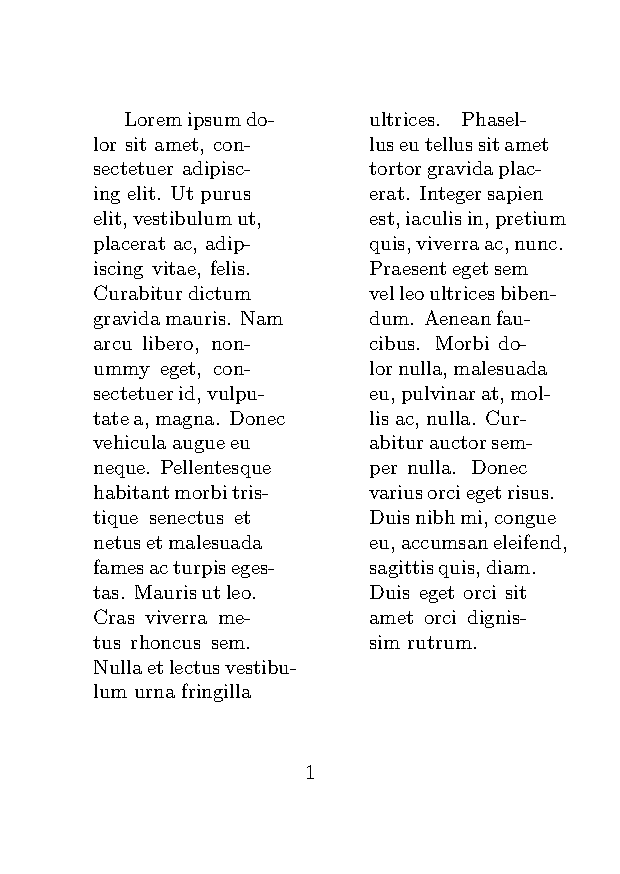
\includegraphics[scale=.6]{images/choix_extensions_exemple_colonnes}
\end{boxedminipage}





\section{Composition à l'italienne (landscape)}



\subsection{En cours de document}

Avec l'extension \mintinline{latex}{lscape} : placer le contenu de la page à l'italienne dans l'environnement \mintinline{latex}{landscape}. Dans ce cas, l'en-tête et le pied de page restent en place comme dans :

\vspace*{1em}
\begin{minipage}{.48\linewidth}
    \begin{minted}{latex}
    \documentclass{report}
    \usepackage[a6paper]{geometry}
    \usepackage{lscape}
    \usepackage{lipsum}
    \begin{document}
    \begin{landscape}
    \section*{A l'italienne}
         \lipsum[1]
    \end{landscape}
    \end{document}
    \end{minted}
\end{minipage}
\begin{boxedminipage}{.48\linewidth}
	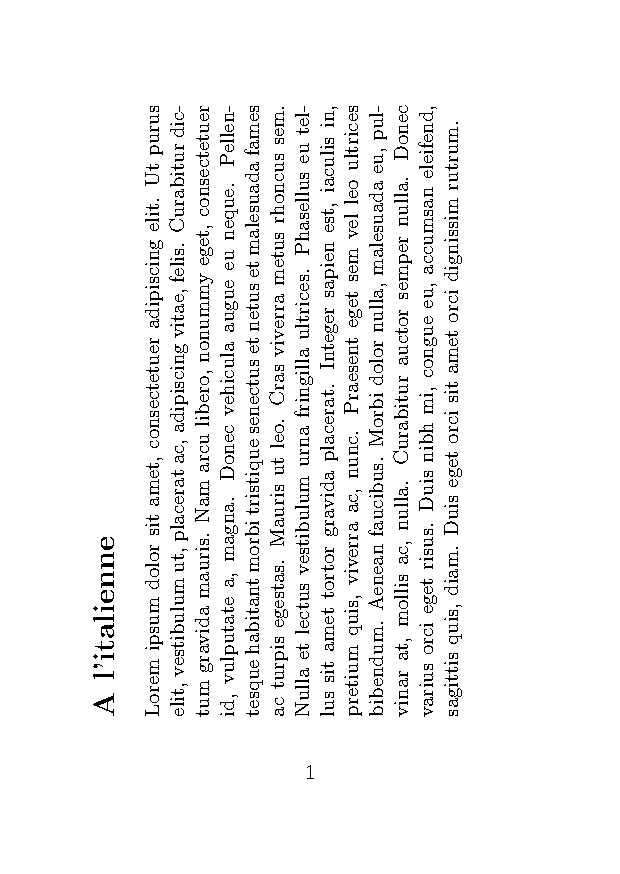
\includegraphics[width=\linewidth]{images/choix_extensions_exemple_lscape}
\end{boxedminipage}



\subsection{Pour tout un document}

Utiliser l'option \mintinline{latex}{landscape} dans l'extension \mintinline{latex}{geometry} : \mintinline{latex}{usepackage[landscape]geometry} :

\vspace{1em}
\begin{minipage}{.48\linewidth}
	\begin{minted}{latex}
    \documentclass{report}
    \usepackage[landscape,a6paper]
         {geometry}
    \usepackage{lipsum}
    \begin{document}
    \lipsum[47]
    \end{document}
	\end{minted}
\end{minipage}
\begin{boxedminipage}{.48\linewidth}
	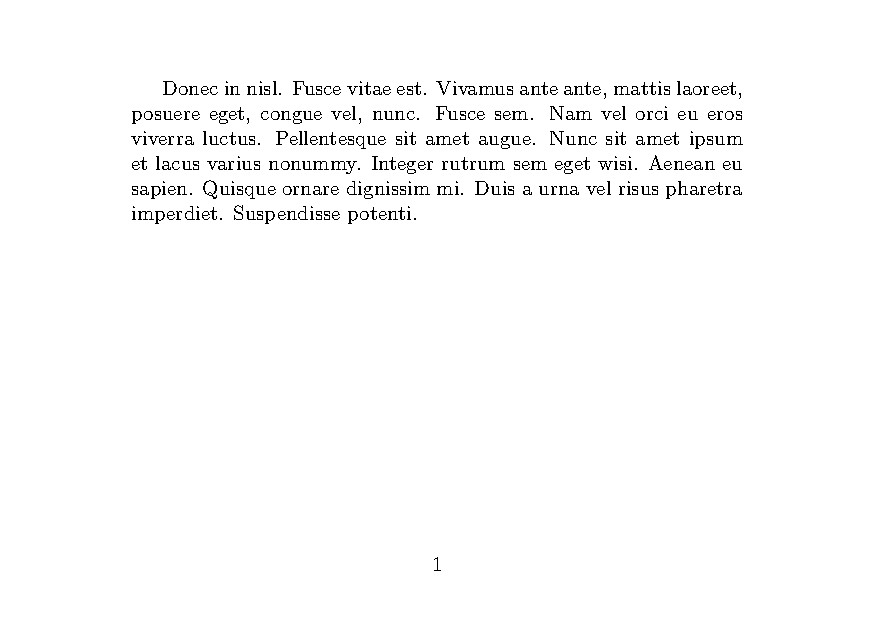
\includegraphics[width=\linewidth]{images/choix_extensions_exemple_landscape}
\end{boxedminipage}






\section{Imprimer en A5}

La gestion du A5 dépend plus de l'imprimante et de ses pilotes que de \LaTeX.

Si l'imprimante support du papier au format A5 : utiliser l'extension \href{}{geometry} avec l'option a5paper : \newline \mintinline{latex}{\usepackage[a5paper]{geometry}}. Ceci génère un PDF au format A5.

Sinon, on peut :
\begin{itemize}
	\item soit garder l'option ci-dessus et, si le driver de l'imprimante le permet, faire tirer deux pages par feuille sans réduction de taille;
	\item soit, ce qui est plus courant, créer des documents en A4 et faire tirer deux pages sur une. Attention à la réduction de taille d'environ \SI{71}{\%} (les fontes en \SI{12}{pt} ressortent environ en \SI{8,5}{pt}).
\end{itemize}
	% !TeX encoding = UTF-8
% !TeX root = choix_extensions.tex
\chapter{Paragraphes spéciaux}
\label{ch:paragraphesSpeciaux}

Certains paragraphes spéciaux sont très fréquents dans nos documents : \emph{Exemples}, \emph{Définition}, \emph{Remarque}, \emph{Théorèmes}\dots \ Une grosse partie du fichier \incmd{preambule_college.sty} sert à définir des raccourcis pour de tels paragraphes. 




\section{Raccourcis pour les définitions}
\label{sec:paragrapheSpecialDefin}

Les commandes suivantes permettent de gérer les définitions :
\begin{enumerate}
	\item \mintinline{latex}{\defin[titre]{paragraphe}} permet de produire un cadre pour une définition;
	\item \mintinline{latex}{\defins[Titre]{Définitions}}) : la même au pluriel;
	\item \mintinline{latex}{\emphdef} permet de mettre en évidence les mots à définir.
\end{enumerate}

\remarque*{
	On peut modifier la numérotation (voir \ref{sec:numerotationParagraphes}), mais pas la supprimer.
}

\begin{LTXexample}[pos=o,width=.4]
\defin{
    Définition
}
\defins{
    Version au \emphdef{pluriel}
}
\defin[titre]{
    Version avec \emphdef{titre} en option
}
\defins[titre]{
    Les \emphdef{deux variantes}
}
\end{LTXexample}





\section{Raccourcis pour des paragraphes fréquents}
\label{sec:paragraphesSpeciauxThmtools}

Le fichier \incmd{preambule_college.sty} présente toute une série de raccourcis pour les paragraphes les plus courants, chacun dans trois variantes (voir l'exemple ci-dessous):
\begin{enumerate}
	\item un titre en option (\mintinline{latex}{\exemple[Titre]{Exemple}});
	\item une version au singulier et une au pluriel (\mintinline{latex}{\exemple} et \mintinline{latex}{\exemples});
	\item une version normale et une étoilée, donc sans numérotation (\lstinline!\exemple*!)
\end{enumerate}

\erreurCourante*{
	Dans le code \LaTeX, il n'est pas possible de laisser une ligne vide dans un de ces environnements : une erreur de compilation est générée (p. ex. \inlatex{Paragraph ended before \probleme was complete.})
}

Les fichiers \incmd{.sty} proposés contiennent la définition des commandes suivantes :
\begin{itemize}[leftmargin=*]
	\begin{multicols}{4}
		\item \mintinline{latex}{\exemple}
		\item \mintinline{latex}{\contreExemple}
		\item \mintinline{latex}{\remarque}
		\item \mintinline{latex}{\exercice}
		\item \mintinline{latex}{\exerciceEtoile}
		\item \mintinline{latex}{\probleme}
		\item \mintinline{latex}{\problemeEtoile}
		\item \mintinline{latex}{\rappel}
		\item \mintinline{latex}{\rappelEtoile}
		\item \mintinline{latex}{\propriete}
		\item \mintinline{latex}{\notionIntuitive}
		\item \mintinline{latex}{\hypothese}
		\item \mintinline{latex}{\these}
		\item \mintinline{latex}{\conclusion}
		\item \mintinline{latex}{\demonstration}
		\item \mintinline{latex}{\notation}
		\item \mintinline{latex}{\algorithme}
		\item \mintinline{latex}{\erreurCourante}
		\item \mintinline{latex}{\bestPractice}
		\item \mintinline{latex}{\astuce}
	\end{multicols}
\end{itemize}

\begin{LTXexample}[pos=o,width=.4]
\exemple{
    Exemple de base
}
\exemples{
    Exemples (au pluriel)
}
\exemple[titre]{
    Exemple avec titre
}
\exemples[titre]{
    Exemple au pluriel avec titre
}
\exemple*{
    Exemple sans numérotation
}
\exemples*{
    Au pluriel sans numérotation
}
\exemple*[titre]{
    Avec titre, sans numérotation
}
\exemples*[titre]{
    Avec titre, au pluriel, sans numérotation
}
\end{LTXexample}

\remarques*{
	\listtopsep
	\begin{enumerate}
		\item Lorsque ces paragraphes débutent immédiatement par une liste (comme c'est le cas pour ce paragraphe-ci), il manque un retour à la ligne. Pour le forcer, voir \ref{sec:listeParSpeciaux}.
		\item Ces paragraphes sont réalisés avec l'extension \href{http://mirror.ctan.org/macros/latex/exptl/thmtools/thmtools.pdf}{thmtools}. La section \ref{sec:numerotationParagraphes} présente comment adapter la numérotation à ses besoins. Pour le reste, cette extension permet de nombreuses variantes de cadre, d'ombrage, de couleurs\dots
		\item Les commandes , \mintinline{latex}{\problemeEtoile} et \mintinline{latex}{\rappelEtoile} servent à faire afficher une étoile dans le document final, par exemple pour indiquer un exercice plus difficile ou un rappel spécial.
	\end{enumerate}
}





\section{Raccourcis pour des paragraphes avec cadres}
\label{sec:paragraphesSpeciauxCadre}

Certains paragraphes sont mis en forme avec des cadres réalisés en \mintinline{latex}{TikZ}\footnote{TikZ est un langage graphique pour \LaTeX.}. Ces commandes sont disponibles en version étoilée (conformément à la syntaxe \LaTeX, les versions étoilées n'ont pas de numérotation) et prennent un titre en option.

\begin{LTXexample}[pos=o,width=.4]
\axiome{
    Un axiome
}
\axiome*{
    Un axiome
}
\end{LTXexample}


Les commandes suivantes sont disponibles :
\begin{multicols}{3}
	\begin{itemize}
		\item \mintinline{latex}{\axiome}
		\item \mintinline{latex}{\theoreme}
		\item \mintinline{latex}{\corollaire}
		\item \mintinline{latex}{\equivalence}
		\item \mintinline{latex}{\regle}
	\end{itemize}
\end{multicols}





\section[Numérotation]{Numérotation des paragraphes spéciaux et références}
\label{sec:numerotationParagraphes}


\subsection[Type de numérotation]{Modifier le type de numérotation}

On peut modifier facilement la numérotation des paragraphes spéciaux dans le fichier \mintinline{latex}{preambule_college.sty}\footnote{Moins facile, mais plus propre : redéfinir le paragraphe spécial dans \mintinline{latex}{preambule_college.sty}.}. Par exemple, la numérotation des rappels recommence à 1 à chaque chapitre à cause du code suivant :

{\small \Verb!\declaretheorem[name=Rappel,style=collegeBase,!{\color{red} \Verb!parent=chapter!}\Verb!]{rappelThm}!}

Pour éviter que la numérotation ne recommence à zéro à chaque chapitre, il suffit d'enlever \mintinline{latex}{parent=chapter}. On peut évidemment mettre autre chose que \mintinline{latex}{chapter} après \mintinline{latex}{parent}. Pour plus de détails, voir la documentation de \href{http://mirror.ctan.org/macros/latex/exptl/thmtools/thmtools.pdf}{thmtools}.



\subsection{Modification de la numérotation}

Les paragraphes spéciaux sont créés à partir d'environnements \mintinline{latex}{theorem}. Par exemple, pour \mintinline{latex}{\exercice}, on voit, dans \mintinline{latex}{preambule_college.sty}, qu'il y a un environnement \mintinline{latex}{exerciceThm}. A cet environnement est associé un compteur de même nom qu'on peut régler avec \mintinline{latex}{\setcounter}.

Par exemple on crée des exercices et on donne ensuite la solution en faisant repartir à zéro le compteur associé :

\begin{LTXexample}[pos=o,width=0.4]
\setcounter{exerciceThm}{8}

\subsubsection{Données}
    \exercice{Neuvième exercice}
    \exercice{Dixième exercice}

\setcounter{exerciceThm}{8}

\subsubsection{Solutions}
    \exercice{Solution de l'exercice 9}
    \exercice{Solution de l'exercice 10}
\end{LTXexample}





\newpage





\subsection{Références vers des paragraphes}

Les paragraphes spéciaux sont, en principe, tous construits sur le même modèle. Les commandes \mintinline{latex}{\rappel} et \mintinline{latex}{\rappels} permettent d'illustrer le principe.

\begin{minipage}{.65\linewidth}
	\begin{minted}{latex}
\rappel{
    \label{rappel1}
    Premier point de référence.
}
\rappels[Rappel avec un titre]{
    \label{rappel2}
    Deuxième point de référence.
}

Faisons référence :
\begin{enumerate}
    \item au premier rappel (le \autoref{rappel1});
    \item seulement à son numéro (le \ref{rappel1});
    \item au nom du deuxième (\nameref{rappel2}).
\end{enumerate}
	\end{minted}
\end{minipage}
\hfill
\begin{boxedminipage}{.34\linewidth}
	\rappel{
		\label{rappel1}
		Premier point de référence.
	}
	\rappels[Rappel avec un titre]{
		\label{rappel2}
		Deuxième point de référence.
	}
	
	Faisons référence :
	\begin{enumerate}
		\item au premier rappel (le \autoref{rappel1});
		\item seulement à son numéro (le \ref{rappel1});
		\item au nom du deuxième (\nameref{rappel2}).
	\end{enumerate}
\end{boxedminipage}





\section{Problèmes connus}



\subsection{Note de bas de page dans un paragraphe spécial}

Lorsqu'un appel de note de bas de page reste collé à un environnement, par exemple dans une définition ou un paragraphe encadré, il est possible de l'envoyer tout de même en bas de page.

\subsubsection{Note mal placée}

\defin{
	Une définition avec une note de bas de page dans le cadre \footnote{Note dans le cadre}
}

Exemple réalisé avec ce code :

\begin{minted}{latex}
\defin{
  Une définition avec une note de bas de page dans le cadre
  \footnote{Note dans le cadre
}
\end{minted}

\subsubsection{Note placée correctement}

\defin{
	Une définition avec une note en bas de page
	\footnotemark
}
\footnotetext{Note de bas de page au bon endroit}
Exemple réalisé avec ce code :

\begin{minted}{latex}
\defin{
  Une définition avec une note en bas de page
  \footnotemark
}
\footnotetext{Note de bas de page au bon endroit}
\end{minted}



\subsection{Problème de filet dans une définition}

\begin{minipage}[t]{.5\linewidth}
	Il arrive que, lorsque la définition se situe en haut d'une page, le filet horizontal coupe le texte au lieu d'arriver juste en dessous comme dans l'exemple ci-contre.
	
	Dans une telle situation, il suffit de mettre un \inlatex{\newpage} juste avant pour forcer un saut de page propre et tout revient dans l'ordre.
\end{minipage}
\hfill
\begin{minipage}[t]{.45\linewidth}
	\vspace{-5ex}
	\defin{
		Lorem ipsum dolor sit amet, consectetur adipiscing elit. Cras fermentum feugiat nisi in condimentum.
		\vspace*{-2ex}
	}
\end{minipage}



\subsection{Erreur "Paragraph ended before <nom> was complete" à la compilation}

Ce message provient d'une ligne vide dans le code, à l'intérieur d'un paragraphe spécial. Par exemple, une ligne vide pour séparer deux \inlatex{\item} dans une liste produit ce message d'erreur. Utiliser \inlatex{\\} au besoin, mais ne pas introduire de ligne vide !





\section{D'autres personnalisations}



\subsection{Avec tcolorbox}

C'est le dernier package arrivé et sans doute le plus intéressant et le plus puissant ! Les autres peuvent être largement ignorés. Un exemple tiré du manuel (de 428 pages quand même\dots)

\begin{LTXexample}[pos=o]
	\begin{tcolorbox}[title=My title,
		colback=red!5!white,
		colframe=red!75!black,
		colbacktitle=yellow!50!red,
		coltitle=red!25!black,
		fonttitle=\bfseries,
		subtitle style={boxrule=0.4pt,
			colback=yellow!50!red!25!white} ]
		This is a \textbf{tcolorbox}.
		\tcbsubtitle{My subtitle}
		Further text.
		\tcbsubtitle{Second subtitle}
		Further text.
	\end{tcolorbox}
\end{LTXexample}


\subsection{Avec thmtools}

A l'aide des exemples de la documentation de \href{http://mirror.ctan.org/macros/latex/exptl/thmtools/thmtools.pdf}{thmtools}, on peut notamment configurer la manière dont fonctionnent le compteur, les références, la couleur de fond, le style de caractères, l'indentation\dots


Il est relativement facile de personnaliser un style de paragraphe spécial, par exemple, pour lui ajouter un fond :

\begin{LTXexample}[pos=o]
    \begin{boxedDefinition}[Exemple]
        Début de la définition
    \end{boxedDefinition}
\end{LTXexample}

Pour créer ce fond, il suffit de créer un nouveau style, par exemple, ici dans le préambule :
\begin{minted}[autogobble]{latex}
  \declaretheoremstyle[notefont=\bfseries,parent=chapter,shaded={bgcolor=yellow}]{exempleStyle}
  \declaretheorem[style=exempleStyle,name=Définition]{boxedDefinition}
\end{minted}



\subsection{Avec mdframed}

L'environnement \mintinline{latex}{mdframed} offre des possibilités simples de faire des encadrés de paragraphes spéciaux, même sur plusieurs pages. On peut ainsi redéfinir des paragraphes spéciaux pour qu'ils aient une allure moins classique.

L'exemple ci-dessous est réalisé avec les options suivantes :

\begin{minted}{latex}
\mdfdefinestyle{exampledefault}{outerlinewidth=5pt,innerlinewidth=0pt,
outerlinecolor=red,roundcorner=5pt}  
\end{minted}

\global\mdfdefinestyle{exampledefault}{%
	outerlinewidth=5pt,	innerlinewidth=0pt, outerlinecolor=red,	roundcorner=5pt
}

\begin{mdframed}[style=exampledefault]
	\lipsum[1-8]
\end{mdframed}
	% !TeX encoding = UTF-8
% !TeX root = choix_extensions.tex
\chapter{Listes}
\label{ch:gestionListes}

Pour gérer finement les listes, rien ne vaut le package \href{http://mirror.ctan.org/macros/latex/contrib/enumitem/enumitem.pdf}{enumitem}. En l'appelant avec l'option \mintinline{latex}{shortlabels} \newline (\mintinline{latex}{\usepackage[shortlabels]{enumitem}}), il est compatible avec l'ancienne extension \mintinline{latex}{enumerate} qui est largement moins puissant.





\section[enumerate]{Énumérations spéciales}



\subsection*{Personnalisation de la numérotation}

\begin{LTXexample}[pos=o]
\begin{enumerate}[a.]
    \item Un
    \item Deux
    \item Trois
\end{enumerate}
\end{LTXexample}

\begin{LTXexample}[pos=o]
\begin{enumerate}[1.]
    \item Un
    \item Deux
    \item Trois
\end{enumerate}
\end{LTXexample}

\begin{LTXexample}[pos=o]
\begin{enumerate}[1)]
    \item Un
    \item Deux
    \item Trois
\end{enumerate}
\end{LTXexample}



\subsection*{Raccourcis}

Le fichier \incmd{preambule_college.sty} contient les commandes suivants : \mintinline{latex}{enuma}, \mintinline{latex}{enum}, \mintinline{latex}{enumpar} :

\begin{LTXexample}[pos=o]
\enuma{
    \item Un
    \item Deux
    \item Trois
}
\end{LTXexample}

\begin{LTXexample}[pos=o]
\enum{
    \item Un
    \item Deux
    \item Trois
}
\end{LTXexample}

\begin{LTXexample}[pos=o]
\enumpar{
    \item Un
    \item Deux
    \item Trois
}
\end{LTXexample}





\section{Régler les espacements}



\subsection{Verticaux}

L'option \mintinline{latex}{itemsep} permet d'aérer la liste et \mintinline{latex}{topsep} règle l'espacement avec le texte avant ou après la liste (il y a encore d'autres paramètres plus pointus dans la documentation d'\mintinline{latex}{enumitem}).

\begin{LTXexample}[pos=o,width=.4]
Texte précédent
\begin{enumerate}[itemsep=.2cm, topsep=.5cm]
    \item Un
    \item Deux
    \item Trois
\end{enumerate}
Texte suivant
\end{LTXexample}



\subsection{Horizontaux}

Pour éviter l'indentation de la liste : \mintinline{latex}{leftmargin=*}. Pour régler l'espacement entre le numéro et le texte : \mintinline{latex}{labelsep=} et la distance voulue.
\begin{LTXexample}[pos=o,width=.4]
Texte précédent
\begin{enumerate}[leftmargin=*, labelsep=1cm]
    \item Un
    \item Deux
    \item Trois
\end{enumerate}
Texte suivant
\end{LTXexample}


Tout aligner horizontalement sur la fin des labels :
\begin{LTXexample}[pos=o,width=.4]
\begin{description}[
    font=\normalfont,
    leftmargin=!,
    labelwidth=\widthof{2000 :}]
    \item[1994 :] Le 1er octobre, le \href{http://www.w3.org}{w3c} est créé pour définir des protocoles \dots
    \item[1995 :] Le web compte 25'000 sites en ligne
\end{description}
\end{LTXexample}





\section{Listes dans un paragraphe spécial}
\label{sec:listeParSpeciaux}

Si un des paragraphes spéciaux des sections \ref{sec:paragrapheSpecialDefin} et \ref{sec:paragraphesSpeciauxThmtools} débute immédiatement pas une liste (sans aucun texte entre le titre du paragraphe spécial et la liste), il manque un retour à la ligne. Le raccourci \mintinline{latex}{\listtopsep} permet de régler le problème :

\begin{LTXexample}[pos=o,width=.4]
\exemples{
      \listtopsep
      \begin{itemize}
             \item Avec
             \item précaution
      \end{itemize}
}
\end{LTXexample}





\newpage





Parfois, il est nécessaire de régler cet espace au cas par cas. On peut le faire :
\begin{enumerate}[a.]
	\item de manière semi-automatique;
		\begin{LTXexample}[pos=o,width=.4]
\exemples{
    \leavevmode
    \vspace*{-\parskip}
    \vspace*{-\baselineskip}
    \begin{itemize}
        \item Avec
        \item précaution
    \end{itemize}
}
		\end{LTXexample}
	
	\item à la main, par exemple ici l'espacement est de \mintinline{latex}{-3ex}.
	   \begin{LTXexample}[pos=o,width=.4]
\exemples{
   \leavevmode
   \vspace*{-3ex}
   \begin{itemize}
       \item Avec
       \item précaution
   \end{itemize}
}
	\end{LTXexample}
\end{enumerate}
	% !TeX encoding = UTF-8
% !TeX root = choix_extensions.tex
\chapter{Gérer les graphiques}
\label{ch:graphiques}





\section{Texte et figure en parallèle}



\subsection{Figure sans légende - raccourcis}

Le fichier \lstinline!preambule_college.sty! contient des raccourcis basés sur les \lstinline!minipage! : \newline
\lstinline!\txtfig{taille_texte en %}{texte}{figure}! et \lstinline!\figtxt{taille_figure en %}{figure}{texte}! :


%\setlength\fboxsep{0pt}
%\setlength{\txtWidth}{(\linewidth - \widthof{\quad}) * \real{.65}}
%\setlength{\figWidth}{\linewidth - \widthof{\quad} - \txtWidth }
%\noindent
%\begin{minipage}[m]{\txtWidth}
%	{Texte en parallèle d'une figure.}
%\end{minipage}% %N.B. le % est nécessaire pour éviter un espace inter-mot supplémentaire entre les minipages
%\hfill
%\begin{minipage}[m]{\figWidth}
%	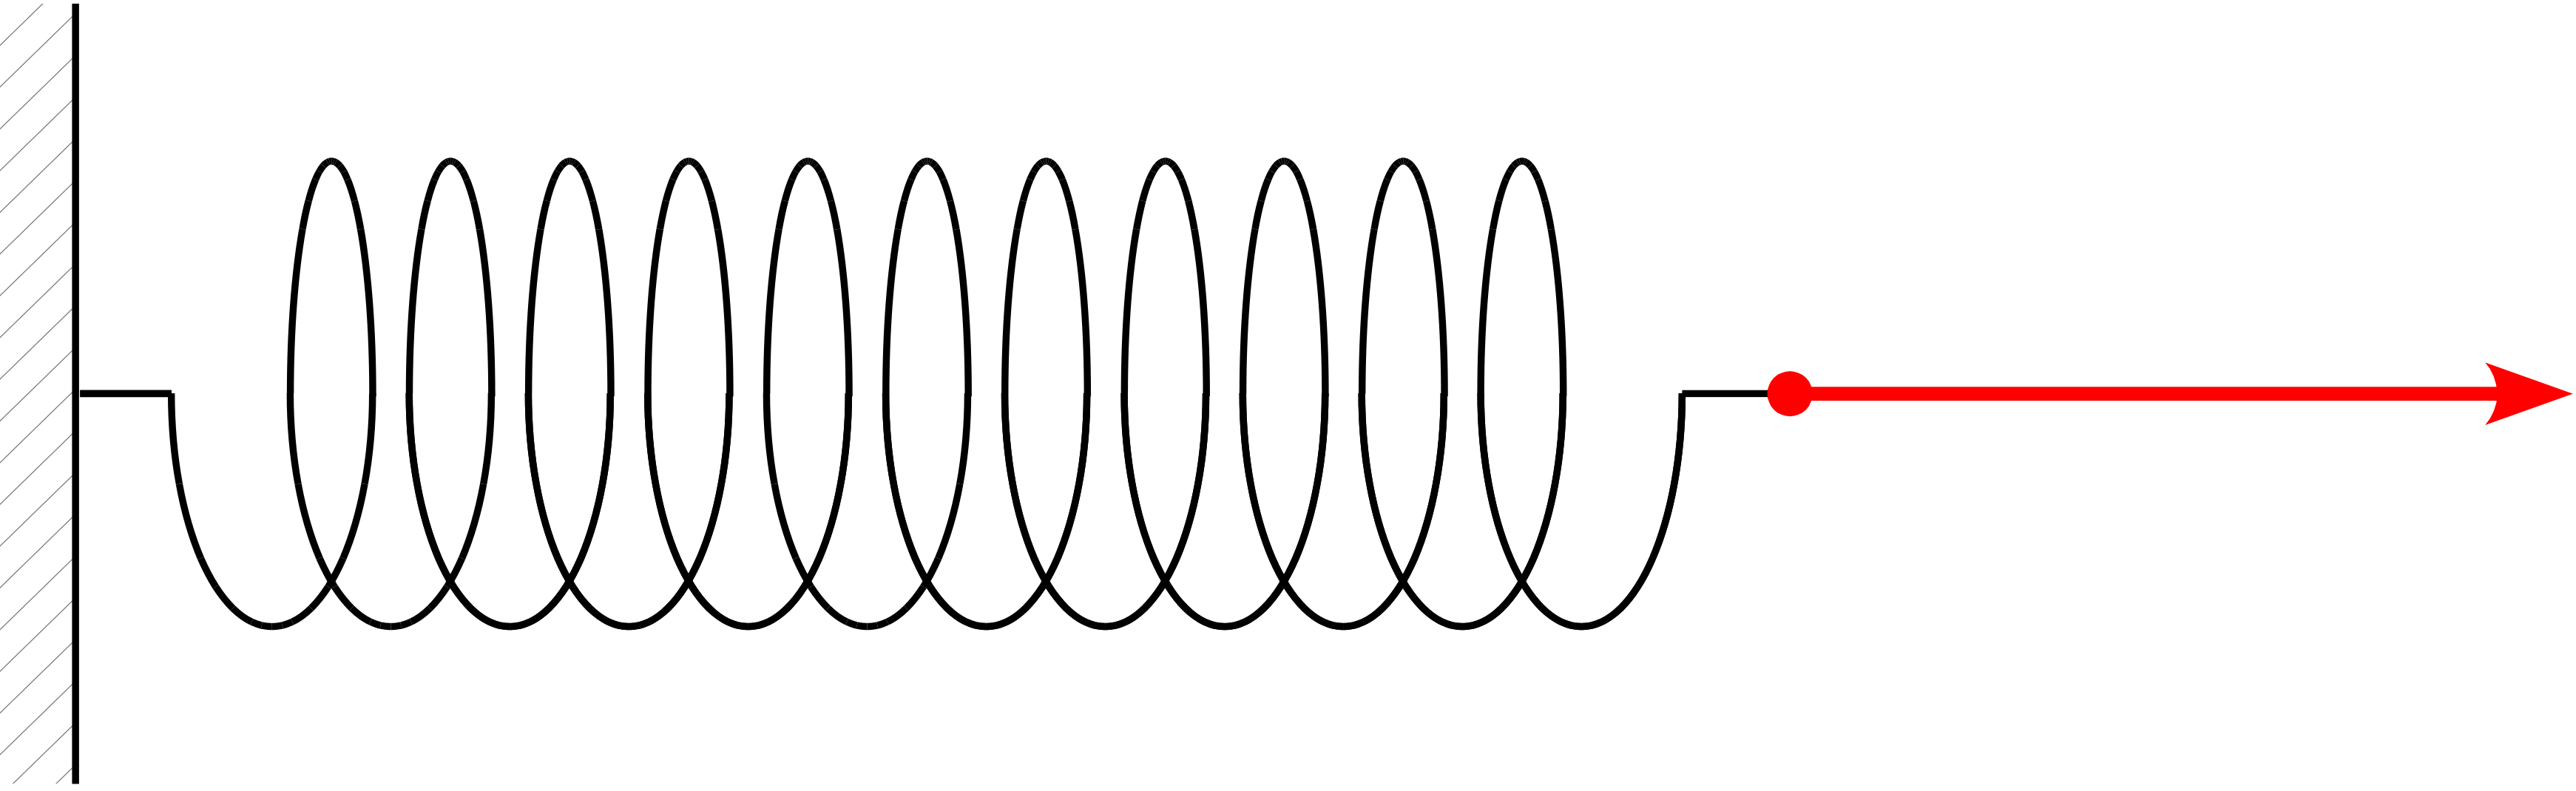
\includegraphics[width=\linewidth]{images/vecteur_force}
%\end{minipage}


\begin{LTXexample}[pos=o]
\txtfig{.65}
  {Texte en parallèle d'une figure.}
  {images/vecteur_force}
\end{LTXexample}

\begin{LTXexample}[pos=o]
\figtxt{.65}
  {images/vecteur_force}
  {Texte en parallèle d'une figure.}
\end{LTXexample}


\subsection{Figure sans légende - à la main}

Presque la même, mais à la main : on peut ainsi jouer sur les paramètres de centrage des minipages. Par exemple, ici avec le paramètre \lstinline![m]! (milieu) :

\begin{LTXexample}[pos=o]
\begin{minipage}[m]{.58\linewidth}
    Texte en parallèle d'une figure.
\end{minipage}% %Un % est nécessaire ici
\hfill
\begin{minipage}[m]{.38\linewidth}
    \centering
%    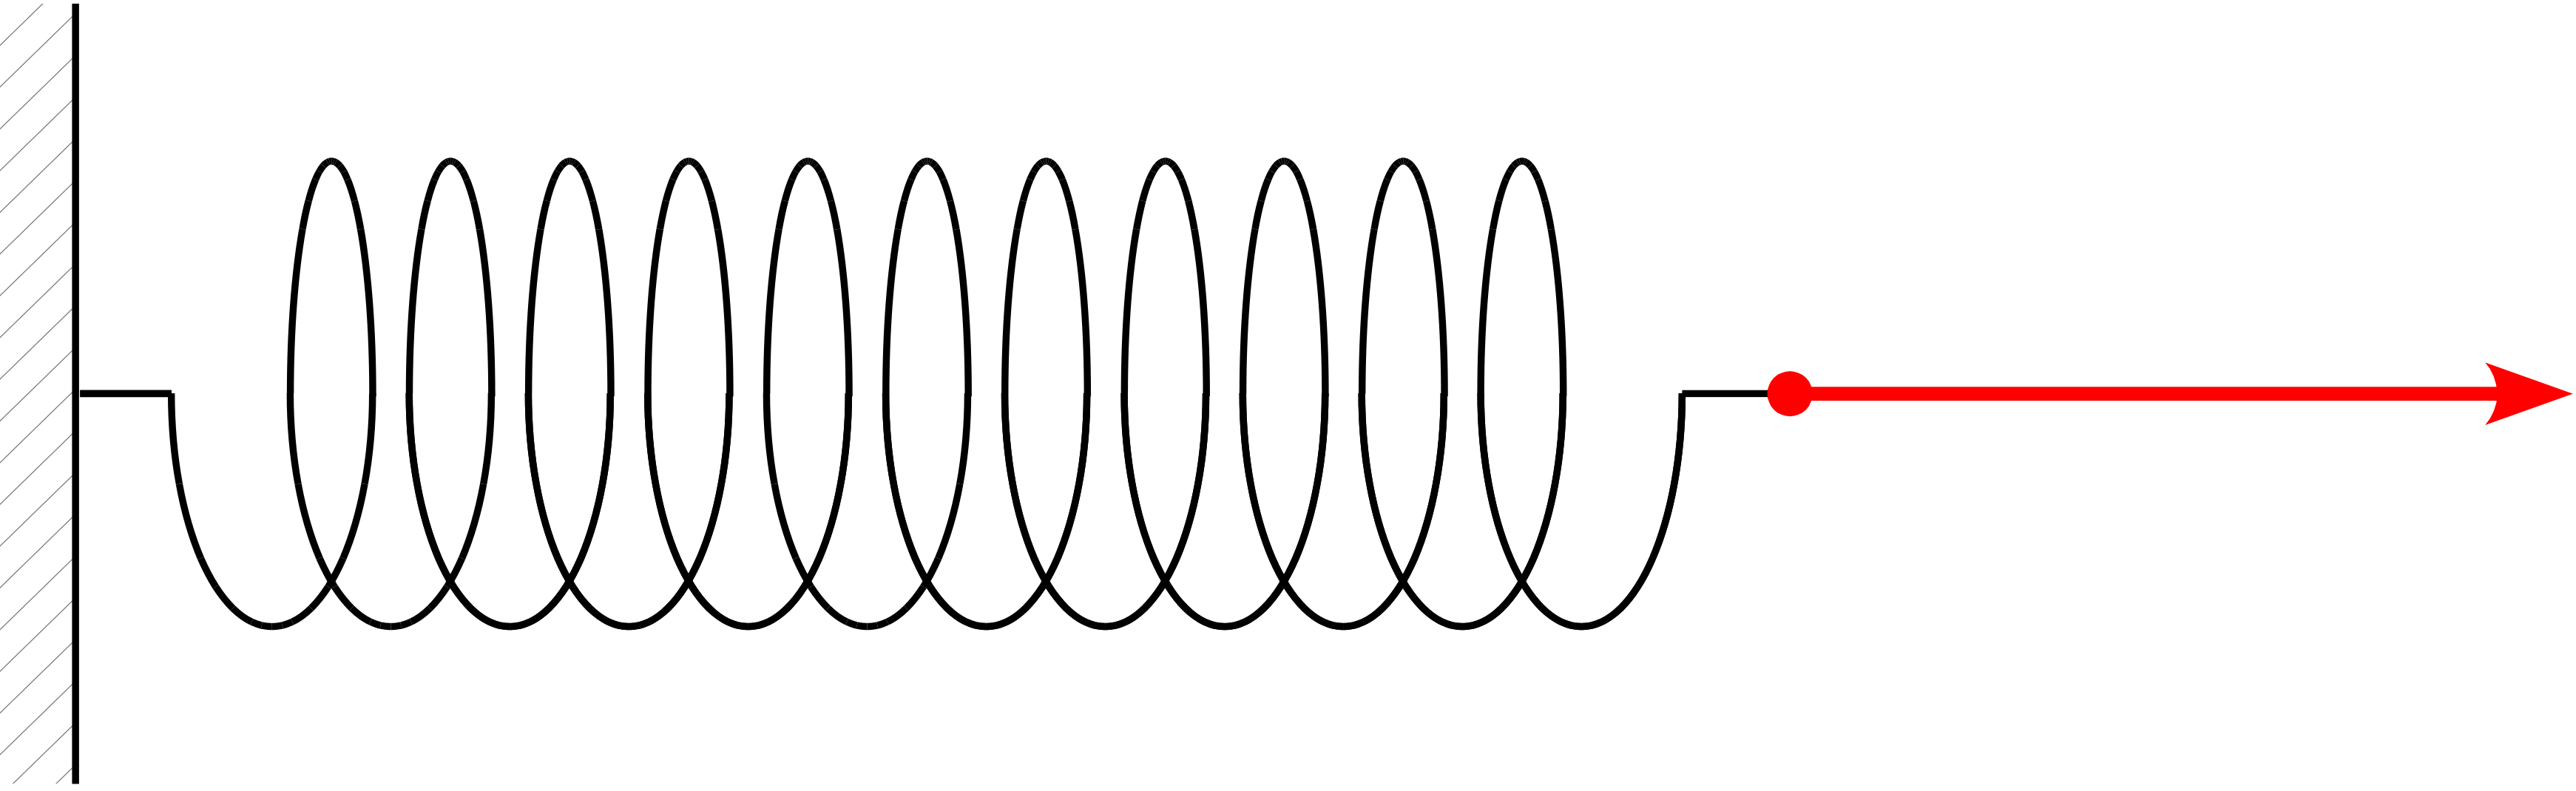
\includegraphics[width=\linewidth]{images/vecteur_force}
\end{minipage}
\end{LTXexample}



\subsection{Figure avec légende}

\begin{LTXexample}[pos=o]
\begin{minipage}[m]{.58\linewidth}
    Texte en parallèle d'une figure.
\end{minipage}% %Un % est nécessaire ici
\hfill
\begin{minipage}[m]{.38\linewidth}
    \centering
%    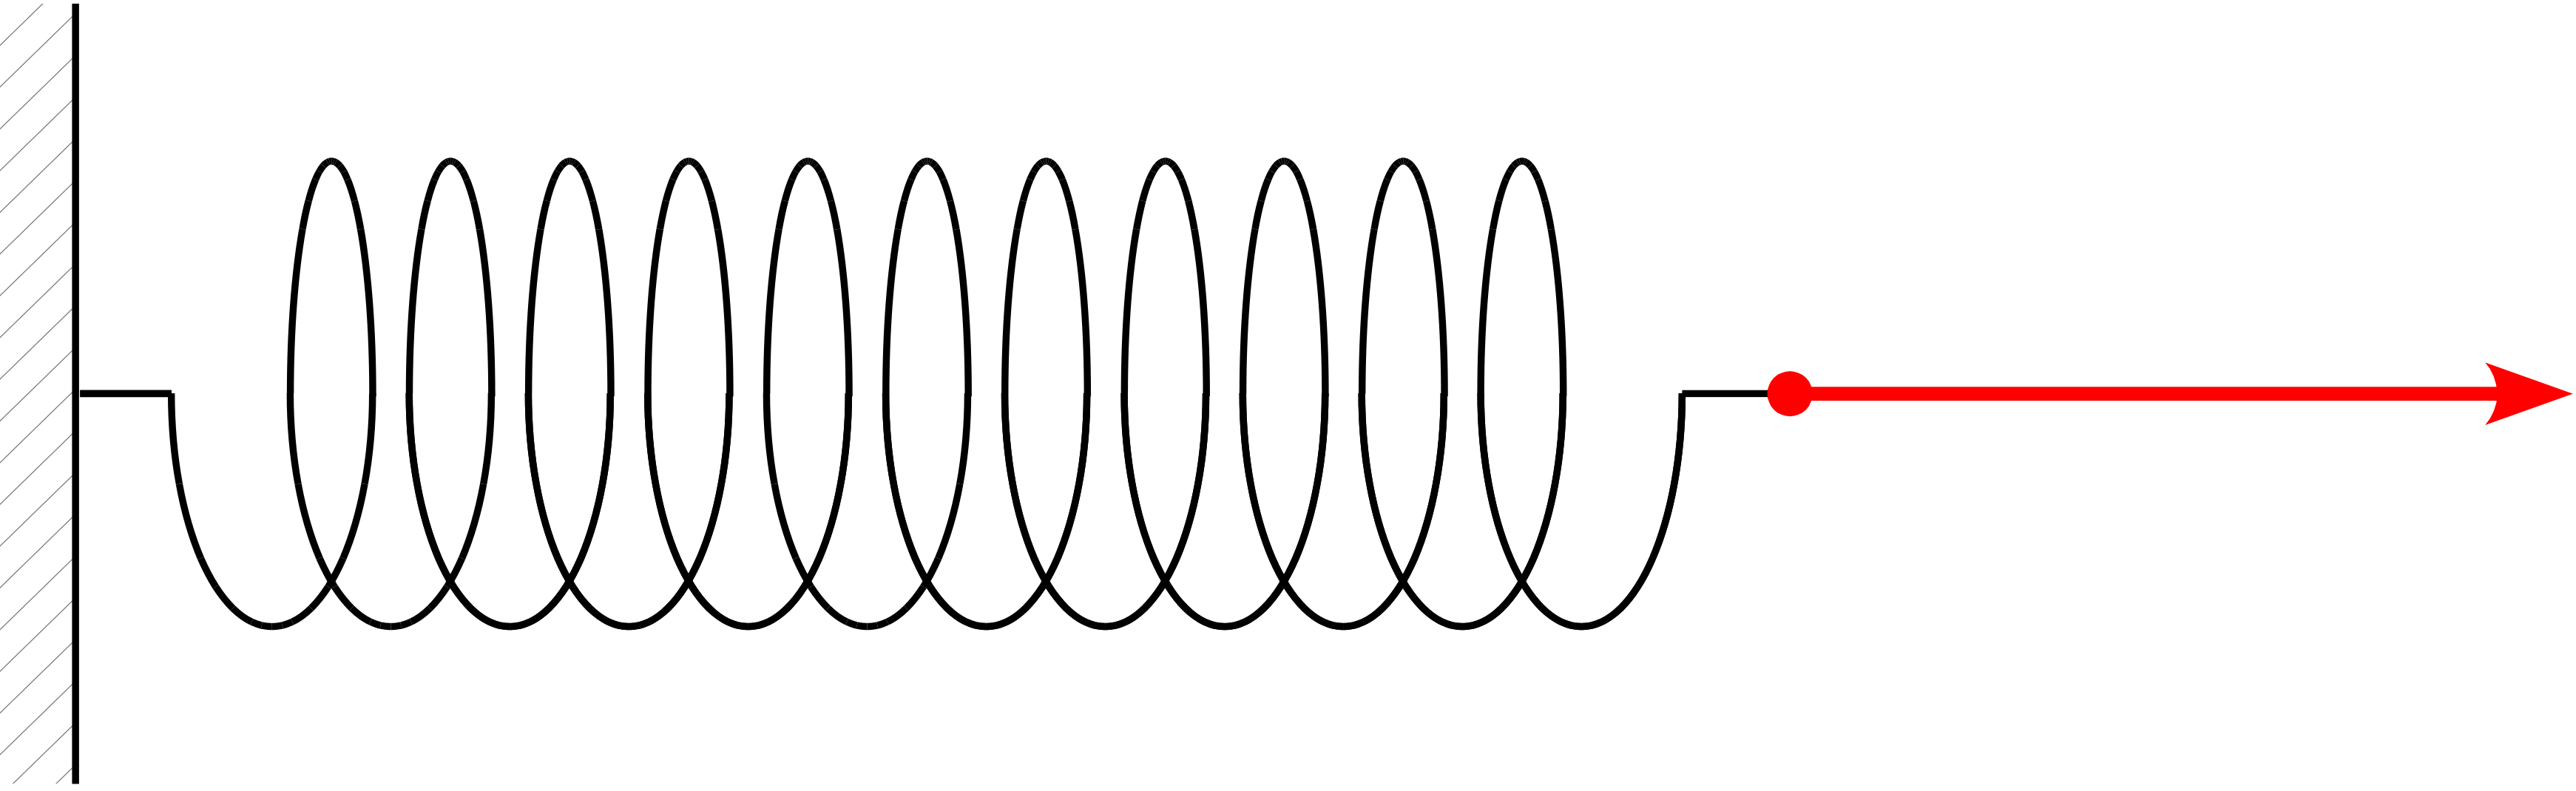
\includegraphics[width=\linewidth]{images/vecteur_force}
    \captionof{figure}{Force}
\end{minipage}
\end{LTXexample}

\remarques*{
	\listtopsep
	\begin{enumerate}
		\item Attention \mintinline{latex}{\captionof{figure}{...}} de l'extension \href{http://www.ctan.org/pkg/caption}{caption} permet d'insérer une légende dans une minipage, mais peut chambouler l'ordre de la numérotation pour les figures à proximité. Il faut vérifier le placement des autres figures autour de celle-ci.
		\item On peut aussi faire ce type de mise en page avec l'extension \mintinline{latex}{float} et \mintinline{latex}{\begin{figure}[H]}, mais ceci n'est pas entièrement compatible avec l'usage de l'extension \mintinline{latex}{minitoc}.
	\end{enumerate}
}





\section{Sous-figures}
\label{sec:textFig}

\begin{minipage}[m]{.48\linewidth}
	\begin{minted}{latex}
\begin{figure}{\linewidth}
  \centering
  \captionsetup{type=figure}
  \subcaptionbox
    {Lentille biconvexe\label{fig:l1}}
    [.45\linewidth]
    {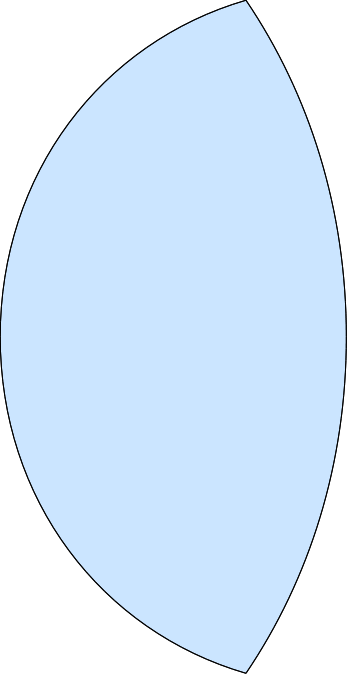
\includegraphics{images/lentille1}
  }
  \quad
  \subcaptionbox
    {Ménisque à bord mince\label{fig:l2}}
    [.45\linewidth]{
    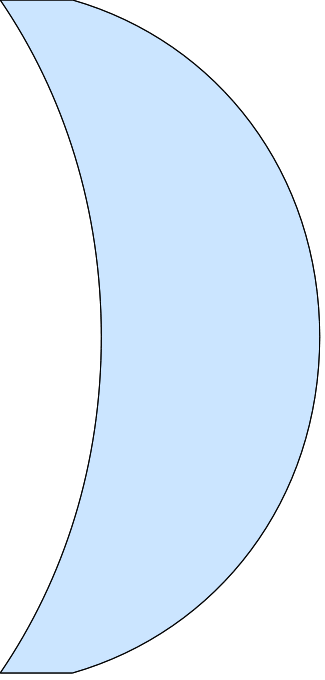
\includegraphics{images/lentille2}
  }
  \caption{Lentilles convergentes
  	\subref{fig:l1} et \subref{fig:l2}}
  \label{fig:lentillesTypes}
\end{figure}
	\end{minted}
\end{minipage}
\hfill
\begin{minipage}[m]{.48\linewidth}
	\begin{figure}[H]%{\linewidth}
		\centering
		\captionsetup{type=figure}
		\subcaptionbox{Lentille biconvexe\label{fig:l1}}[.45\linewidth]{
			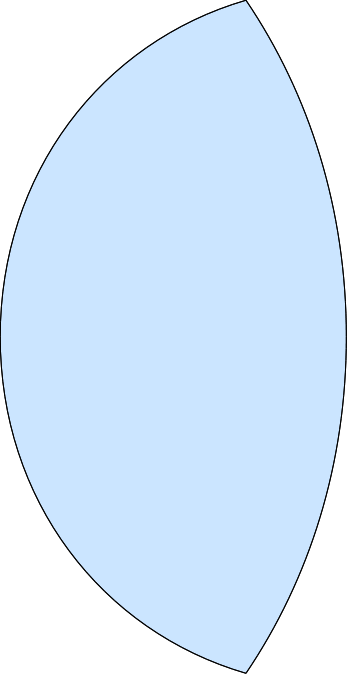
\includegraphics{images/lentille1}
		}
		\quad
		\subcaptionbox{Ménisque à bord mince\label{fig:l2}}[.45\linewidth]{
			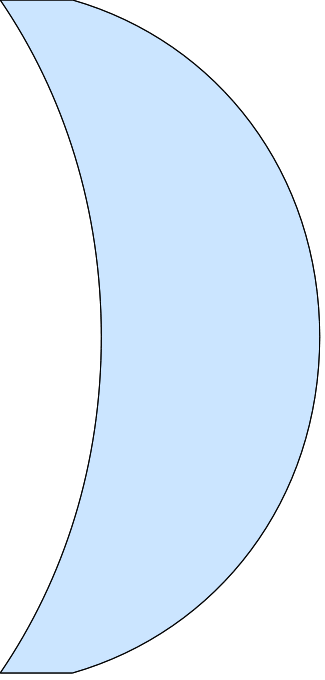
\includegraphics{images/lentille2}
		}
		\caption{Lentilles convergentes
			\subref{fig:l1} et \subref{fig:l2}}
		\label{fig:lentillesTypes}
	\end{figure}
\end{minipage}


\remarque*{
	L'extension \mintinline{latex}{\href{http://mirror.ctan.org/macros/latex/contrib/subfig/subfig.pdf}{subfig}} permet aussi de faire ce type de mise en page, mais elle a des incompatibilités avec \mintinline{latex}{hyperref}.
%	\begin{minipage}[m]{.48\linewidth}
%		\begin{minted}{latex}
%	\begin{figure}[H]
%	  \centering
%	  \subfloat[Lentille biconvexe]{
%	    \includegraphics[width=2.5cm]
%	      {images/lentille1}}
%	    \label{a}
%	   }
%	  \quad
%	  \subfloat[Ménisque à bord mince]{
%	    \includegraphics[width=2.5]
%	      {images/lentille2}
%	     }
%	    \label{b}
%	  }
%	  \caption{Lentilles convergentes}
%	  \label{fig:lentillesTypes}
%	\end{figure}
%		\end{minted}
%	\end{minipage}
%	\hfill
%	\begin{minipage}[m]{.48\linewidth}
%		\begin{figure}[H]
%			\centering
%		  	\subfloat[Lentille biconvexe]{
%		    \makebox[2.5cm]{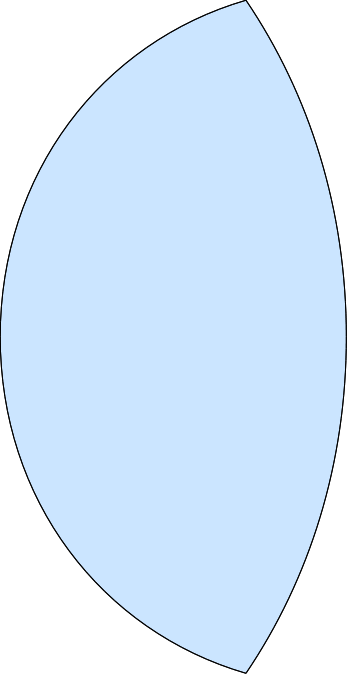
\includegraphics{images/lentille1}}
%		    \label{a}
%		  }
%		  \quad
%		  \subfloat[Ménisque à bord mince]{
%		    \makebox[2.5cm]{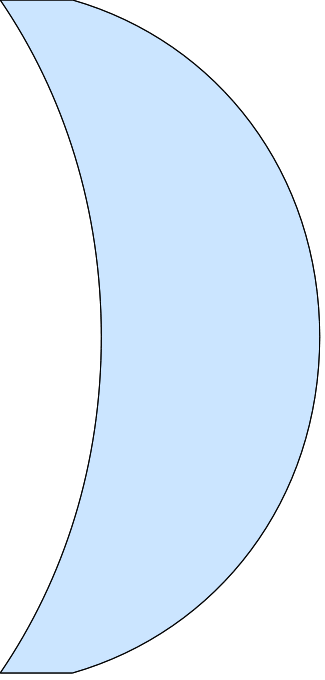
\includegraphics{images/lentille2}}
%		    \label{c}
%		  }
%		  \caption{Lentilles convergentes}
%		  \label{fig:lentillesTypes}
%		\end{figure}
%	\end{minipage}
}





\section{Alignement horizontal des minipages}

Si on veut aligner correctement le haut de deux \mintinline{latex}{minipages} (deux options \mintinline{latex}{[t]}), il se peut que le résultat ne soit pas celui escompté (voir code ci-après) :

\begin{LTXexample}[pos=o,width=.4]
\begin{minipage}[t]{4cm}
  \[
    \cS_{B'CC'} = \cS_{B'BC'}
  \]
\end{minipage}
\hfill
\begin{minipage}[t]{2cm}
  \centering
  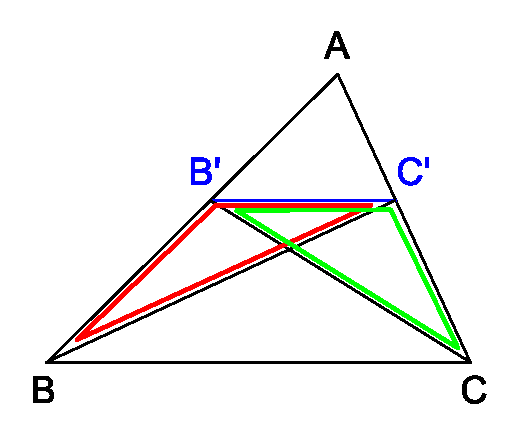
\includegraphics
    [width=.8\linewidth]
    {images/Thales_thm_Thales_dem_01}
\end{minipage}
\end{LTXexample}

Pour éviter cela, il suffit de rajouter \mintinline{latex}{\vspace{0pt}} dans la deuxième \mintinline{latex}{minipage} de manière à donner un point de référence correct à \LaTeX.

\begin{LTXexample}[pos=o,width=.4]
\begin{minipage}[t]{4cm}
  \[
    \cS_{B'CC'} = \cS_{B'BC'}
  \]
\end{minipage}
\hfill
\begin{minipage}[t]{2cm}
  \vspace{0pt}
  \centering
  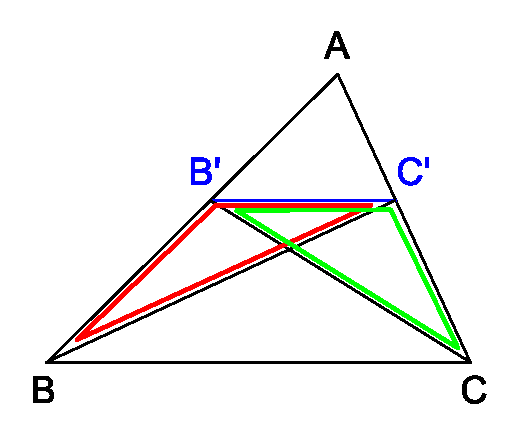
\includegraphics
    [width=.8\linewidth]
    {images/Thales_thm_Thales_dem_01}
\end{minipage}
\end{LTXexample}
	% !TeX encoding = UTF-8
% !TeX root = choix_extensions.tex
\chapter{Tableaux}





\section{Aérer les tableaux}



\subsection{Augmenter la hauteur de ligne}

Pour augmenter la hauteur des cellules, uniquement vers le haut, utiliser \mintinline{latex}{extrarowheight{...}}. Remarque : en mettant le \mintinline{latex}{extrarowheight{...}} dans un environnement \mintinline{latex}{center}, cela en limite l'effet à ce tableau.

\begin{LTXexample}[pos=o,width=.3\linewidth]
\begin{center}
  \setlength\extrarowheight{12pt}
  \begin{tabular}{|p{5ex}|l|}
    \hline
    P1 & $a^ma^n = a^{m + n}$ \\
    \hline
    P2 & $\left( {a^m} \right)^n = a^{mn}$ \\
    \hline
  \end{tabular}
\end{center}
\end{LTXexample}



\subsection{Augmenter la hauteur de ligne et centrer verticalement}

Pour augmenter la taille des cellules de manière centrée : insérer une réglure verticale de largeur nulle et décalée verticalement (p. ex. \mintinline{latex}{\rule[-2ex]{0pt}{5.5ex}}) :

\begin{LTXexample}[pos=o,width=.3\linewidth]
\begin{center}
  \begin{tabular}{|>{\rule[-2ex]{0pt}{5.5ex}}p{5ex}|c|}
    \hline
    P1 & $a^ma^n = a^{m + n}$ \\
    \hline
    P2 & $\left( {a^m} \right)^n = a^{mn}$ \\
    \hline 
  \end{tabular} 
\end{center}
\end{LTXexample}

C'est la version que propose l'\incmd{assistant tableau} de TeXstudio.





\section{Centrage horizontal et vertical}

Sur une ligne du tableau, pour faire aligner verticalement deux cellules : utiliser le type de colonne \mintinline{latex}{m{taille}}. Pour faire simultanément un centrage horizontal : rajouter un \mintinline{latex}{\centering} dans chaque cellule (en utilisant l'option de colonne \mintinline{latex}{>{}}).

\erreurCourante*{
	Il n'est plus possible alors d'utiliser \mintinline{latex}{\\} pour terminer une ligne, il faut utiliser explicitement \mintinline{latex}{\tabularnewline}.
}

\begin{LTXexample}[pos=o,width=.25\linewidth]
\begin{center}
  \begin{tabular}{|>{\centering}m{1cm}|>{\centering}m{1cm}|}
    \hline 
    {\Huge $\updownarrow$} & Flèche \tabularnewline
    \hline
    Flèche & {\Huge $\updownarrow$} \tabularnewline 
    \hline
  \end{tabular} 
\end{center}
\end{LTXexample}





\section{Tableaux mathématiques}
\label{sec:tableauxMaths}

Pour faire des tableaux en mode mathématique, utiliser l'environnement \mintinline{latex}{IEEEeqnarray} (voir \ref{sec:alignementEquations}). Comme alternative, il y a aussi \mintinline{latex}{array}. On peut en ajuster la hauteur de ligne avec \mintinline{latex}{extrarowheight} et l'espace inter colonne avec \mintinline{latex}{\arraycolsep} comme dans l'exemple ci-dessous :
\begin{LTXexample}[pos=o]
\[
  \setlength\extrarowheight{4pt}
  \setlength{\arraycolsep}{0pt}
  \begin{array}{rrrrr<{~}|>{~}l}
    4x^4 & -2x^3 & +0x^2 & +5x & -7 \hspace{0.3cm} & 2x^2+0x-3\\
    \cline{6-6}
    -4x^4 & -0x^3 & +6x^2 & & & 2x^2-x+3\\
    \cline{1-3}
    & -2x^3 & +6x^2 & +5x & & \\
    & +2x^3 & +0x^2 & -3x & & \\
    \cline{2-4}
    & & 6x^2 & +2x & -7 &\\
    & & -6x^2 & -0x & +9 &\\
    \cline{3-5}
    & & & 2x & +2 & \\
  \end{array}
\]
\end{LTXexample}

Noter aussi l'utilisation de la commande \mintinline{latex}{\cline} pour la réalisation de filets horizontaux sur une seule partie du tableau.





\section{Pense-bête}

Déclarer directement plusieurs colonnes de même type, fusion de cellules, filet partiel : 
\begin{LTXexample}[pos=o,width=.4]
\setlength\extrarowheight{1ex}
\begin{tabular}{|*{10}{c|}}
  \hline
  1 & 2 & 3 & 4 & 5 & 6 & 7 & 8 & 9 & 10 \\
  \cline{1-5}
  \multicolumn{5}{|c|}{Cinq colonnes} & \multicolumn{5}{c|}{Cinq autres} \\
  \cline{0-4}
  1 & 2 & 3 & 4 & 5 & 6 & 7 & 8 & 9 & 10 \\
  \hline
  1 & 2 & 3 & \multirow{2}{*}[2ex]{4} & 5 & 6 & 7 & 8 & 9 & 10 \\
  \cline{1-3} \cline{5-10}
  1 & 2 & 3 &  & 5 & 6 & 7 & 8 & 9 & 10 \\
  \hline
  1 & 2 & 3 & 4 & 5 & 6 & 7 & 8 & 9 & 10 \\
  \hline
  1 & 2 & 3 &
    \multicolumn{3}{c|}{\multirow{2}*{4 \ 5 \ 6}}
    & 7 & 8 & 9 & 10 \\
  \cline{1-3} \cline{7-10}
  1 & 2 & 3 &
    \multicolumn{3}{c|}{} & 7 & 8 & 9 & 10 \\
  \hline
  1 & 2 & 3 & 4 & 5 & 6 & 7 & 8 & 9 & 10 \\
  \hline
\end{tabular}
\end{LTXexample}





\section{Tables professionnelles}

Avec l'extension \href{https://www.ctan.org/pkg/booktabs}{booktabs.sty}, on peut faire des tables correspondant aux standards typographiques professionnels :

\begin{LTXexample}
\begin{tabular}{@{}llc@{}} \toprule
    $P$ & $Q$ & $P \;et\; Q$ \\ \midrule
    $\cV$ & $\cV$ & $\cV$ \\
    $\cV$ & $\cF$ & $\cF$ \\
    $\cF$ & $\cV$ & $\cF$ \\
    $\cF$ & $\cF$ & $\cF$ \\ \bottomrule
\end{tabular}
\end{LTXexample}





\section{Numéroter les lignes d'un tableau}

On définit la commande \inlatex{\rownumber} en préambule : 

\begin{minted}[autogobble]{latex}
	\preto\tabular{\setcounter{magicrownumbers}{0}}
	\newcounter{magicrownumbers}
	\newcommand\rownumber{\stepcounter{magicrownumbers}\arabic{magicrownumbers}}
\end{minted}

\begin{LTXexample}
\begin{tabular}{|l|c|}
	N° & Contenu \\
	\hline
	\rownumber & un \\
	\rownumber & deux \\
	\rownumber & trois
\end{tabular}
\end{LTXexample}





\section{Redéfinir les espacement dans un tableau}

\begin{minipage}{.9\linewidth}
	\begin{minted}[autogobble,breaklines]{latex}
        \renewcommand{\arraystretch}{3}
        \newcolumntype{M}[1]{>{\centering\arraybackslash}m{#1}}
        \begin{tabular*}{\textwidth}{@{\extracolsep{\fill}}l*{2}{M{.15\linewidth}}M{.2\linewidth}M{.25\linewidth}}
          \toprule
          \textbf{Suite} & \textbf{Définition} & \textbf{Raison} & \textbf{Terme général} & \parbox{\linewidth}{\textbf{Somme partielle des $\symbf{n}$ premiers termes}} \\
          \addlinespace
          \midrule
          Arith. & $u_{n+1} = u_n + r$ & $r = u_{n+1} - u_n$ & $u_n = u_1 + (n-1) \cdot r$ & $S_n = n \cdot \dfrac{u_1+u_n}{2}$ \\
          Géom. & $u_{n+1} = u_n \cdot r$ & $r = \dfrac{u_{n+1}}{u_n}$ & $u_n = u_1 \cdot r^{n-1}$ & $S_n = u_1 \cdot \dfrac{1-r^n}{1-r}$ \\
          \addlinespace[2ex]
          \bottomrule
        \end{tabular*}
	\end{minted}
\end{minipage}

\begin{center}
	\renewcommand{\arraystretch}{3}
	\newcolumntype{M}[1]{>{\centering\arraybackslash}m{#1}}
	\begin{tabular*}{\textwidth}{@{\extracolsep{\fill}}l*{2}{M{.15\linewidth}}M{.2\linewidth}M{.25\linewidth}}
		\toprule
		\textbf{Suite} & \textbf{Définition} & \textbf{Raison} & \textbf{Terme général} & \parbox{\linewidth}{\textbf{Somme partielle des $\symbf{n}$ premiers termes}} \\
		\addlinespace
		\midrule
		Arith. & $u_{n+1} = u_n + r$ & $r = u_{n+1} - u_n$ & $u_n = u_1 + (n-1) \cdot r$ & $S_n = n \cdot \dfrac{u_1+u_n}{2}$ \\
		Géom. & $u_{n+1} = u_n \cdot r$ & $r = \dfrac{u_{n+1}}{u_n}$ & $u_n = u_1 \cdot r^{n-1}$ & $S_n = u_1 \cdot \dfrac{1-r^n}{1-r}$ \\
		\addlinespace[2ex]
		\bottomrule
	\end{tabular*}
\end{center}
	% !TeX encoding = UTF-8
% !TeX root = choix_extensions.tex
\chapter{Maths}





\section{Extensions mathématiques particulièrement utiles}

Entre TeXstudio et le fichier \mintinline{latex}{preambule_college.sty}, il y a tout ce qu'il faut pour bien faire :
\begin{itemize}
	\item L'extension de \emph{l'American Mathematical Society} (AMS) \href{https://www.ctan.org/pkg/amsmath}{amsmath}, \href{https://www.ctan.org/tex-archive/fonts/amsfonts}{amsfonts}, \href{https://www.ctan.org/pkg/amsopn}{amsopn}.
	\item Les extensions suivantes sont très pratiques et méritent le coup d'{\oe}il :
		\begin{enumerate}
			\item  \href{https://www.ctan.org/tex-archive/macros/latex/contrib/IEEEtran/}{IEEEtran}
			\item \href{https://www.ctan.org/pkg/siunitx}{siunitx}
			\item \href{https://www.ctan.org/tex-archive/macros/latex/contrib/braket}{braket}
			\item \href{https://www.ctan.org/pkg/esvect}{esvect}.
		\end{enumerate}
	\item Avec TeXStudio, la plupart des symboles et des environnement mathématiques sont accessibles directement depuis les barres d'outils et le menu \mintinline{latex}{Math}.
\end{itemize}





\section{Paragraphes mathématiques spéciaux}

Pour mémoire (voir \ref{ch:paragraphesSpeciaux}), les paragraphes mathématiques les plus courants sont disponibles sous forme de raccourcis :
\begin{multicols}{3}
	\begin{itemize}
		\item \mintinline{latex}{\defin}
		\item \mintinline{latex}{\theoreme}
		\item \mintinline{latex}{\axiome}
		\item \mintinline{latex}{\hypothese}
		\item \mintinline{latex}{\these}
		\item \mintinline{latex}{\conclusion}
		\item \mintinline{latex}{\demonstration}
		\item \mintinline{latex}{\corollaire}
		\item \mintinline{latex}{\algorithme}
		\item \mintinline{latex}{\consequence}
	\end{itemize}
\end{multicols}

Ce qui donne en pratique :
\begin{multicols}{2}
	\defin[Titre]{A \emphdef{définir}}
	\theoreme[Titre]{Exemple}
	\axiome[Titre]{Exemple}
	\hypothese[Titre]{Exemple}
	\these[Titre]{Exemple}
	\conclusion[Titre]{Exemple}
	\demonstration[Titre]{Exemple}
	\corollaire[Titre]{Exemple}
	\algorithme[Titre]{Exemple}
\end{multicols}





\section{Alignements d'équations}
\label{sec:alignementEquations}

Pour les alignements plus précis, l'extension \href{http://mirror.ctan.org/macros/latex/contrib/IEEEtran/IEEEtran_HOWTO.pdf}{IEEEtran} fournit tous les outils nécessaires.

En particulier, on utilise l'environnement \mintinline{latex}{IEEEeqnarray} pour les alignements complexes. La syntaxe est similaire à celle d'un environnement \mintinline{latex}{tabular} ou \mintinline{latex}{array} (voir \ref{sec:tableauxMaths}).

Ainsi, on obtient : 
\[
	\begin{IEEEeqnarraybox}[][c]{rCrCl}
		\left.
		\begin{IEEEeqnarraybox}[\IEEEeqnarraystrutmode][c]{rCl?l}
			AB &=& CD & \text{(hyp)}\\
			OA &=& OD &(=r)\\
			OB &=& OC &(=r)
		\end{IEEEeqnarraybox}
		\, \right\}
		& \quad \xRightarrow{\parbox{.7cm}{\centering\scriptsize cas 3 iso}} \quad
		& BOA &\cong& DOC \\
		& \quad \xRightarrow{\parbox{1.5cm}{\centering\scriptsize thm angles au centre}} \quad
		& \wideparen{AB} &\cong& \wideparen{CD}
	\end{IEEEeqnarraybox}
\]

avec le code suivant :

\begin{minted}{latex}
\[
  \begin{IEEEeqnarraybox}[][c]{rCrCl}
    \left.
    \begin{IEEEeqnarraybox}[\IEEEeqnarraystrutmode][c]{rCl?l}
      AB &=& CD & \text{(hyp)}\\
      OA &=& OD &(=r)\\
      OB &=& OC &(=r)
    \end{IEEEeqnarraybox}
    \, \right\}
    & \quad \xRightarrow{\parbox{.7cm}{\centering\scriptsize cas 3 iso}} \quad
    & BOA &\cong& DOC \\
    & \quad \xRightarrow{\parbox{1.5cm}{\centering\scriptsize thm angles au
    centre}} \quad
    & \wideparen{AB} &\cong& \wideparen{CD}
  \end{IEEEeqnarraybox}
\]
\end{minted}

Dans cet environnement, on peut regrouper des colonnes avec \mintinline{latex}{\IEEEeqnarraymulticol}. Dans l'exemple suivant, on l'utilise pour aligner \mintinline{latex}{[AM] côté commun} :
\[
	\begin{IEEEeqnarraybox}[][c]{rCrCl?r}
		\left.
		\begin{IEEEeqnarraybox}[\IEEEeqnarraystrutmode][c]{rCl?l}
			\sphericalangle BAM &=& \sphericalangle MAC & ([AM) = b_{\alpha}) \\
			AB &=& AC & \text{(hyp)} \\
			\IEEEeqnarraymulticol{4}{c}{
				\left[AM\right] \text{côté commun}
			}
		\end{IEEEeqnarraybox}
		\, \right\}
		& \quad	\xRightarrow{\parbox{.7cm}{\centering\scriptsize cas 1 iso}} \quad &
		ABM &\cong& ACM \\
		& \quad \xRightarrow{\smash[t]{\text{déf}}} \quad &
		\sphericalangle CBA &=& \sphericalangle ACB &\qedhere
	\end{IEEEeqnarraybox}
\]

obtenu avec le code suivant :

\begin{minted}{latex}
\[
--- Le début du code a été omis ---
  \begin{IEEEeqnarraybox}[\IEEEeqnarraystrutmode][c]{rCl?l}
    \sphericalangle BAM &=& \sphericalangle MAC & ([AM) = b_{\alpha}) \\
    AB &=& AC & \text{(hyp)} \\
    \IEEEeqnarraymulticol{4}{c}{
      \left[AM\right] \text{côté commun}
    }
  \end{IEEEeqnarraybox}
--- La fin du code a été omise ---
\]
\end{minted}



Voir les détails dans le paragraphe sur \mintinline{latex}{IEEEeqnarray} dans \href{http://mirror.ctan.org/info/lshort/french/lshort-fr.pdf}{Une courte (?) introduction à \LaTeX$2\epsilon$} et dans la documentation de \href{http://mirror.ctan.org/macros/latex/contrib/IEEEtran/IEEEtran_HOWTO.pdf}{IEEEtran}.

Pour les cas simples, on peut utiliser \mintinline{latex}{array} (voir \ref{sec:tableauxMaths}). Dans tous les cas, il faut absolument éviter la commande \mintinline{latex}{eqnarray}).





\newpage





\section{Alignements d'exercices}
\label{sec:alignementExercices}

Pour composer des exercices sur plusieurs colonnes, on peut numéroter les exercices par colonne ou par ligne. Généralement, l'utilisation de l'espace est meilleure si on numérote par colonne.



\subsection{Numérotation en colonne (standard)}

Ce résultat est obtenu avec le code ci-dessous :
\exercice*{
	Résoudre :
	\begin{enumerate}[itemsep=1ex]
		\begin{multicols}{2}
			\item $\log_2(x) = 5$ 
			\item $2^{\ln(x)} = 3$ 
			\item $\log_3\left(\log_2(x)\right) = \num{0.5}$
			\item $\ln\left(x^2+3x+1\right) = -2$	
			\item $\log_3\left(x^2-x-1\right) = 1$
			\item $\log_x(5) = 2$
			\item $2\log(x-2)=\log(2x-4)$
			\item $\log_x\left(\dfrac{1}{3}\right)=2$
		\end{multicols}
	\end{enumerate}
}

\begin{minted}[gobble=1,tabsize=2]{latex}
	\exercice*{
		Résoudre :
		\begin{enumerate}[itemsep=1ex]
			\begin{multicols}{2}
				\item $\log_2(x) = 5$ 
				\item $2^{\ln(x)} = 3$ 
				\item $\log_3\left(\log_2(x)\right) = \num{0.5}$
				\item $\ln\left(x^2+3x+1\right) = -2$		
				\item $\log_3\left(x^2-x-1\right) = 1$
				\item $\log_x(5) = 2$
				\item $2\log(x-2)=\log(2x-4)$
				\item $\log_x\left(\dfrac{1}{3}\right)=2$
			\end{multicols}
		\end{enumerate}
	}
\end{minted}

\remarque*{
	De cette manière l'espace est utilisé au mieux, mais les expressions dans les deux colonnes ne sont pas forcément alignées : ce n'est pas un tableau\dots
}



\subsection{Numérotation en colonne sur peu de lignes}

S'il y a peu de lignes et que certaines expressions sont verticalement bien plus grandes que d'autres, des décalages verticaux gênants peuvent apparaître avec \inlatex{multicols}. Dans ce cas, on force l'alignement horizontal en ne tenant pas compte de la hauteur des expressions mathématiques (avec \inlatex{\smash}) et en gérant les espaces interlignes avec \inlatex{itemsep} en option de l'environnement \inlatex{enumerate} :

Par exemple :

\exercice*{
	Soit l'ensemble $E$ des six fonctions suivantes de $\R \smallsetminus \set{0;1}$ vers $\R\smallsetminus \set{0;1}$ :
	\begin{enumerate}[itemsep=2ex]
		\begin{multicols}{3}
			\item[] $\smash{f_1 : x \mapsto x}$
			\item[] $\smash{f_2 : x \mapsto \dfrac{1}{x}}$
			\item[] $\smash{f_3 : x \mapsto 1-x}$
			\item[] $\smash{f_4 : x \mapsto \dfrac{1}{1-x}}$
			\item[] $\smash{f_5 : x \mapsto \dfrac{x-1}{x}}$
			\item[] $\smash{f_6 : x \mapsto \dfrac{x}{x-1}}$
		\end{multicols}
	\end{enumerate}
	Montrer que $(E,\circ)$ est un groupe. Est-il abélien ?
}

Produit par le code :

\begin{minted}[gobble=1,tabsize=2]{latex}
	\exercice{
		Soit l'ensemble $E$ des six fonctions suivantes de $\R \smallsetminus \set{0;1}$ vers $\R\smallsetminus \set{0;1}$ :
		\begin{enumerate}[itemsep=2ex]
			\begin{multicols}{3}
				\item[] $\smash{f_1 : x \mapsto x}$
				\item[] $\smash{f_2 : x \mapsto \dfrac{1}{x}}$
				\item[] $\smash{f_3 : x \mapsto 1-x}$
				\item[] $\smash{f_4 : x \mapsto \dfrac{1}{1-x}}$
				\item[] $\smash{f_5 : x \mapsto \dfrac{x-1}{x}}$
				\item[] $\smash{f_6 : x \mapsto \dfrac{x}{x-1}}$
			\end{multicols}
		\end{enumerate}
		Montrer que $(E,\circ)$ est un groupe. Est-il abélien ?
	}
\end{minted}



\subsection{Numérotation en une ligne}

Pour les alignement en une seule ligne, on peut se passer de \inlatex{multicols} et utiliser directement les environnements étoilés de l'extension \inlatex{enumitem} :

Par exemple :

\exercice*{
	Résoudre : \\[1ex]
	\begin{enumerate*}[itemjoin=\hfill,label=\arabic*),afterlabel=\quad]
		\item $\log_3\left(x^2-x-1\right) = 1$
		\item $\log_x(5) = 2$
		\item $2\log(x-2)=\log(2x-4)$
		\item $\log_x\left(\dfrac{1}{3}\right)=2$
	\end{enumerate*}
}

Produit par le code

\begin{minted}[gobble=1,tabsize=2]{latex}
\exercice*{
	Résoudre : \\[1ex]
	\begin{enumerate*}[itemjoin=\hfill,label=\arabic*),afterlabel=\quad]
		\item $\log_3\left(x^2-x-1\right) = 1$
		\item $\log_x(5) = 2$
		\item $2\log(x-2)=\log(2x-4)$
		\item $\log_x\left(\dfrac{1}{3}\right)=2$
	\end{enumerate*}
}
\end{minted}

\remarque*{
	Pour générer des listes d'exercices dont la numérotation est en ligne, on peut utiliser l'extension \href{https://www.ctan.org/pkg/tasks}{tasks}.
}





\section{Nombres avec unités}

Pour les unités, l'extension \href{http://mirror.ctan.org/macros/latex/contrib/siunitx/siunitx.pdf}{siunitx} offre des fonctionnalités très pratiques :
\begin{LTXexample}[pos=o,width=.4]
Unités indifféremment en mode text, \SI{25}{kJ} ou maths, $E = \SI{25}{kJ}$ \\
Notation scientifique : \SI{4.35e-12}{kg} \\
Unité seule : \si{\degree} \\
Nombre seul : \num{25,3}
\end{LTXexample}



\subsection*{Réglages}

\href{http://mirror.ctan.org/macros/latex/contrib/siunitx/siunitx.pdf}{siunitx} permet de gérer l'apparence des nombres et des unités de manière centrale. Ici, le fichier les options définies dans le fichier \mintinline{latex}{preambule_college.sty} sont : \\

\begin{minipage}{.10\linewidth}
	~
\end{minipage}
\begin{minipage}{.75\linewidth}
	\begin{minted}[autogobble,linenos]{latex}
	  \sisetup{
	    input-digits = 0123456789\dots,
	    output-decimal-marker={.},
	    exponent-product = \cdot,
	    inter-unit-product = \ensuremath{{ } \cdot { }}
	  }
	\end{minted}
\end{minipage}

Ces réglages servent (par ligne) :
\begin{itemize}[leftmargin=!]
	\item[2] pouvoir mettre un \dots \ dans une quantité numérique;
	\item[3] utiliser une virgule décimale dans les nombres;
	\item[4] utiliser un . au lieu d'un x pour la multiplication dans les notations scientifiques;
	\item[5] noter les unités comme dans le "Formulaires et Tables".
\end{itemize}



\attention Dans le SI il n'est pas admis de noter des exposants à virgule, par exemple $10^{2.3}$. Les dernières versions de \incmd{siunitx} vérifient ceci et empêche des écritures du type \inlatex{e2.3}.





\section{Réponses optionnelles aux exercices}

Dans les exercices, on peut lier une réponse à chaque question et la faire afficher avec l'option de compilation \mintinline{latex}{reponse}. Pour cela, le préambule du document doit contenir \mintinline{latex}{\usepackage[reponse]{optional}}. Ceci permet d'activer les raccourcis suivants de  \incmd{preambule_college.sty} :

\begin{enumerate}
	\item \mintinline{latex}{\rep{expression}} : une réponse (expression mathématique requise en argument);
	\item \mintinline{latex}{\rept{text}} : une réponse sous forme de texte (mais pas de liste);
	\item \mintinline{latex}{\repl{liste}} : une réponse texte, y.c. sous forme de liste (basé sur minipage);
	\item \mintinline{latex}{\repn{valeur}} : une réponse numérique, en particulier à virgule basée sur \mintinline{latex}{\num} de l'extension \incmd{siunitx};
	\item \mintinline{latex}{\repSI{valeur}{unité}} : une réponse basée sur \mintinline{latex}{\SI} de l'extension \incmd{siunitx};
	\item \mintinline{latex}{\repNewline} : un \mintinline{latex}{\newline} seulement actif avec les réponses.
\end{enumerate}

\begin{minipage}{.63\linewidth}
	\begin{minted}{latex}
\documentclass{report}
\usepackage{preambule_college}
\usepackage[reponse]{optional}
\begin{document}
\begin{enumerate}
  \begin{multicols}{2}
    \item $\sqrt{6400} =$ $\rep{80}$
    \item Une année-lumière. \repSI{9,45e12}{km}
    \item $(2x+1)(4x-5)=0$\repNewline
      $\rep{S=\Set{-\dfrac{1}{2}; \dfrac{5}{4}}}$
    \item $\num{0,005} \cdot \num{0,06}
      = \repn{3e-4}$
    \item $(x+2)(x-3)(2x-5)(x-\sqrt{3})=0$\repNewline
      \repl{$S_{\N}=\Set{3}$\\ $S_{\Z}=\Set{-2; 3}$\\
        $S_{\Q}=\Set{-2; 3; \cfrac{5}{2}}$\\
        $S_{\R}=\Set{-2; 3; \cfrac{5}{2}; \sqrt{3}}$
      }
  \end{multicols}
\end{enumerate}
\end{document}
	\end{minted}
\end{minipage}
\hfill
\begin{minipage}{.35\linewidth}
	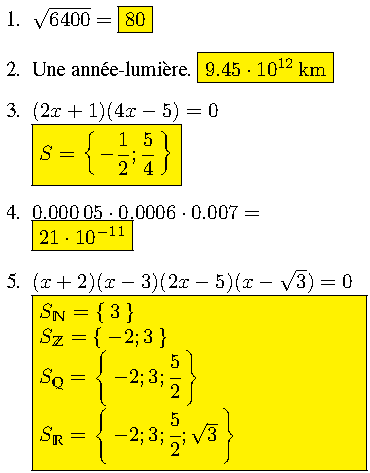
\includegraphics{images/choix_extensions_exemple_reponses}
\end{minipage}




\section{Symboles}



\subsection{Trouver efficacement des symboles}

Pour trouver des symboles, on peut :
\begin{enumerate}
	\item Utiliser les barres d'outils de TeXstudio.
	\item Parcourir \href{https://www.ctan.org/tex-archive/info/symbols/comprehensive/}{The Comprehensive \LaTeX Symbol List}. Pour cela, il faut soit connaître le nom anglais du symbole, soit être patient\dots
	\item Le site \href{http://webdemo.myscript.com}{\url{http://webdemo.myscript.com}} propose l'outil "Web Equation" qui permet d'écrire à la main une formule et vous donne la traduction \LaTeX.
	\item Dessiner son symbole dans \href{http://detexify.kirelabs.org/classify.html}{detexify}. Detexify est aussi disponible pour iOS et pour Android, ce qui permet de dessiner à la main et non à la souris !
\end{enumerate}



\subsection{Symboles mathématiques en gras}

Pour mettre un symbole en gras, par exemple dans un titre, on utilise \inlatex{\symbf} avec l'extension \incmd{unicode-math}. 
\begin{LTXexample}[pos=o,width=.3]
\subsubsection*{Le nombre $\pi$}
\subsubsection*{Le nombre ${\symbf\pi}$}
\end{LTXexample}

Anciennement, on utilisait soit \inlatex{\mathbf{}}, soit \inlatex{\bm} de l'extension du même nom.


Pour mettre un symbole en gras dans un titre de chapitre, dans l'en-tête, mais pas dans la table des matières : \mintinline{latex}{{\boldmath\SI[detect-weight]{0}{\degree}}}



\vspace*{\topsep}
\subsection{Symboles faits maison}

Le fichier \mintinline{latex}{preambule_college.sty} comporte des raccourcis permettant de faire des symboles divers non définis en standard :
\begin{LTXexample}[pos=o,width=.3]
\nRe                \\% pas en relation avec
\nsubset            \\% non inclus
\nbot               \\% non perpendiculaire
\nLeftrightarrow	\\% non équivalent
\vide               \\% ensemble vide un peu plus joli...
\ie                 \\% id est 
\de                 \\% °, basé sur siunitx
\Hyp                \\% pour introduire une hypothèse
\The                \\% pour introduire une thèse
\Dem                \\% pour introduire une démonstration
\nondef				  % pour les valeurs "non définies" dans les tables de signe
\end{LTXexample}



\subsection{Divers symboles}


\subsubsection{Symboles pour les arcs}

En utilisant directement les accents de la police mathématique\footnote{Il faut donc que la police les ait\dots \ Pour l'instant, seules celles accessibles par les commandes \inlatex{\mathversion} de \incmd{preambule_personnalisation.sty} fonctionnent correctement.}.

\begin{LTXexample}[pos=o,width=.3]
$\wideparen{ABC}$
\end{LTXexample}


En utilisant l'extension \href{https://www.ctan.org/pkg/mathtools}{mathtools} :
\begin{LTXexample}[pos=o,width=.3]
$\xRightarrow{\parbox{.7cm}{\centering\scriptsize cas 3}}$
\end{LTXexample}


\subsubsection{Symboles récupérés}

Certains symboles sont liés à une police de caractère, notamment \mintinline{latex}{Palatino}. Le fichier \mintinline{latex}{prambule_college.sty} en récupère quelques-uns sans qu'il n'y ait besoin de changer toute la police de caractères :

\begin{LTXexample}[pos=o,width=.3]
$\varparallel$  \\ % parallèle (penché à droite)
$\nvarparallel$    %non parallèle (penché à droite)
\end{LTXexample}





\section{Raccourcis divers}



\subsection{Fractions}

Pour varier le style des fractions, on utilise les extensions AMS et \href{http://mirror.ctan.org/macros/latex/contrib/l3packages/xfrac.pdf}{xfrac}.
\begin{LTXexample}[pos=o,width=.3]
$\dfrac{1}{2}$ \\[1ex]
$\sfrac{1}{2}$ \\[1ex]
$\cfrac{1}{2}$
\end{LTXexample}

\mintinline{latex}{\cfrac} se comporte bien dans les fractions de fraction. Par ailleurs, pour les cas désespérés dans lesquels l'espacement autour de la barre de fraction doit être réglé finement :
\begin{LTXexample}[pos=o,width=.15]
$\genfrac{}{}{0.9pt}{0}{3\cdot \dfrac52 + \dfrac39} {2-\dfrac{-8}{12}}$
\end{LTXexample}




\subsection{Barrer des expressions}

Pour barre une expression mathématique, on peut utiliser l'extension \href{http://mirror.ctan.org/macros/latex/contrib/cancel/cancel.pdf}{cancel}.

\begin{LTXexample}[pos=o,width=.3]
$\dfrac{2x^{\cancel{2}}}{\cancel{x}}$
\end{LTXexample}



\subsection{Valeur absolue, norme}

Ces raccourcis définis selon \href{http://mirror.ctan.org/macros/latex/contrib/mh/mathtools.pdf}{mathtools} permettent de gérer l'espacement horizontal et la hauteur des barres, automatiquement ou à la main (avec \inlatex{\big}, \inlatex{\Big}, \inlatex{\bigg} ou \inlatex{\Bigg}) :

\begin{LTXexample}[pos=o,width=.3]
$\abs*{\frac{3}{4}}$ \\[1ex]
$\norm*{\frac{x^2}{y^2}}$ \\[1ex]
$\abs[\Big]{\frac{3}{4}}$ \\[1ex]
$\norm[\bigg]{\frac{x^2}{y^2}}$
\end{LTXexample}



\subsection{Réciproque}

\begin{LTXexample}[pos=o,width=.3]
$\recip{G}$
\end{LTXexample}



\subsection{Barre sur une expression}

Pour avoir un peu plus d'espace entre la barre et l'expression :
\begin{LTXexample}[pos=o,width=.3]
$\ovline{P \text{ ou } Q}$
\end{LTXexample}

Pour la composition des nombres périodiques :
\begin{LTXexample}
	$\SI[parse-numbers=false]{0,\overline{1234}}{m^2}$
\end{LTXexample}




\subsection{Ensembles et intervalles}
Les ensembles sont faits avec \mintinline{latex}{\set} (hauteur fixe) et \mintinline{latex}{\Set} (hauteur variable) de l'extension \incmd{braket} :

\begin{LTXexample}[pos=o,width=.3]
$\set{x \in \N | x^2-1=0}$ \\[1ex]
$\Set{x \in \N | \dfrac{x}{2} \in \N}$
\end{LTXexample}

Pour les intervalles : toujours utiliser \mintinline{latex}{\left} et \mintinline{latex}{\right} avec les crochets, sinon il y a un problème d'espacement avant et après les \mintinline{latex}{[]}. Ca permet aussi de les retrouver plus facilement dans le code.

\remarque*{
	Barre verticale hors des ensembles : \mintinline{latex}{\mid} est la même chose que \mintinline{latex}{\;|\;}, et dans un \mintinline{latex}{\left... \right...} on peut utiliser \mintinline{latex}{\middle} à la place de \mintinline{latex}{\mid} pour avoir une hauteur variable. Sinon, \mintinline{latex}{\;\big|\;}.
}



\subsection{Systèmes d'équations}

Réalisés avec l'extension \incmd{IEEEtrantools} pour pouvoir gérer finement les alignements :

\begin{LTXexample}[pos=o,width=.3]
$\left\{ \,
\begin{IEEEeqnarraybox}[][c]{cCc}
  \IEEEstrut
  \frac{x}{2} - \frac{1}{3} &>& \frac{2-x}{4} \\[1ex]
  3x(x-2) &\leqslant& x^2 - 2x
  \IEEEstrut
\end{IEEEeqnarraybox}
\right.$
\end{LTXexample}

\begin{LTXexample}[pos=o,width=.3]
$\left\{ \,
\begin{IEEEeqnarraybox}[][c]{cCcCc?c}
  \IEEEstrut
  7x &-& 2y &=& 4 & (1)\\
  -4x &+& 5y &=& 17 & (2)
  \IEEEstrut
\end{IEEEeqnarraybox}
\right.$
\end{LTXexample}

Voir ci-dessous les extraits de la documentation de \incmd{IEEEeqnarraybox} :


\subsubsection{IEEEstrut}

\inlatex{\IEEEstrut[height][depth][decl]} \\
decl : The optional argument is for commands that are to be executed within the environment, but before the alignment actually begins.


\subsubsection{Descripteurs de colonnes}

\setlength\extrarowheight{3pt}
\begin{tabular}{|c|l||c|l|}
	\hline
	I.D. & Description & I.D. & Description \tabularnewline
	\hline
	l & left math & v & vertical rule \tabularnewline
	c & centered math & vv & two vertical rule \tabularnewline
	r & right math & V & double vertical rule \tabularnewline
	L & left math with ords & VV & two double vertical rule \tabularnewline
	C & centered math with ords & h & horizontal rule\tabularnewline
	R & right math with ords & H & double horizontal rule\tabularnewline
	s & left text & x & empty \tabularnewline
	t & centered text & X & empty math \tabularnewline
	u & right text & & \tabularnewline
	\hline
\end{tabular}


\subsubsection{Descripteurs des séparations}

\begin{tabular}{|c|l||c|l|}
	\hline
	I.D. & Description & I.D. & Description \tabularnewline
	\hline
	! & $-\sfrac{1}{6}$ em & . & \mintinline{latex}{0.5\arraycolsep} \tabularnewline
	, & $\sfrac{1}{6}$ em  & / & \mintinline{latex}{1.0\arraycolsep} \tabularnewline
	: & $\sfrac{2}{9}$ em  & ? & \mintinline{latex}{2.0\arraycolsep} \tabularnewline
	; & $\sfrac{5}{18}$ em  & * & 9pt plus 1fil\tabularnewline
	' & 1 em & + & 1000pt minus 1000pt\tabularnewline
	" & 1 em & - & 0 pt\tabularnewline
	\hline
\end{tabular}


\subsubsection{Espacement des lignes les tableaux}
Pour gérer l'espacement des lignes dans un \mintinline{latex}{IEEEeqnarray} :
\begin{enumerate}
	\item \mintinline{latex}{\IEEEvisiblestrutstrue} pour voir les struts invisibles;
	\item \mintinline{latex}{\IEEEeqnarraystrutsize} and \mintinline{latex}{\IEEEeqnarraystrutsizeadd} pour gérer la hauteur, à placer dans \newline \mintinline{latex}{\begin{IEEEeqnarraybox}[\IEEEeqnarraystrutsize{2ex}{0ex}]}
\end{enumerate}



\subsection{Limites}

\begin{LTXexample}[pos=o,width=.3]
\Lim{1}{2}    %lim
\Limd{1}{2}   %lim plus (ou à droite)
\Limg{1}{2}   %lim moins (ou à gauche)
\end{LTXexample}



\subsection{Vecteurs}

Pour les flèches sur les vecteurs, on utilise l'extension \href{http://mirror.ctan.org/macros/latex/contrib/esvect/esvect.pdf}{esvect}. En appelant l'extension avec une option, on peut choisir la forme de la flèche, ici le \mintinline{latex}{d} : \mintinline{latex}{\usepackage[d]{esvect}} (voir la documentation de \href{http://mirror.ctan.org/macros/latex/contrib/esvect/esvect.pdf}{esvect} pour plus de détail).

Les commandes de base sont : 
\begin{LTXexample}[pos=o,width=.3]
Vecteur quelconque  : $\vv{m}$ ou $\ve{m}$\\
Vecteur avec indice : $\vv*{e}{1}$
\end{LTXexample}

Raccourcis pour les vecteurs courants (avec ou sans les \$) :
\begin{LTXexample}[pos=o,width=.3]
$\va$   $\vb$ $\vc$  $\vd$  $\vn$ $\vu$ \\
$\vvv$ $\vo$ $\veu$ $\ved$ $\vet$
\end{LTXexample}

Raccourcis pour les vecteurs à deux (d) ou trois (t) composantes, avec des crochets :
\begin{LTXexample}[pos=o,width=.3]
$\compd{1}{2}$       %2 composantes
$\compt{1}{2}{3}$   %3 composantes
$\comb{1}{2}{3}$     %3 composantes avec [] brackets
\end{LTXexample}



\subsection{Matrices et déterminants}

\begin{LTXexample}[pos=o,width=.4]
$\matd{1}{2}{3}{4}$
$\matt{1}{2}{3}{4}{5}{6}{7}{8}{9}$
$\detd{1}{2}{3}{4}$
$\dett{1}{2}{3}{4}{5}{6}{7}{8}{9}$
\end{LTXexample}

Si on doit colorer de matrices, il vaut mieux utiliser les modules de TikZ.

\begin{LTXexample}[pos=o,width=.4]
\[
\begin{tikzpicture}
  \matrix (C){
    1 & -2 & 1  \\
    0 & 2  & -8 \\
    5 & 0  & -5 \\
 };
 \node[right=0 of C] (F) {$\cdot$};
 \matrix[right=0.1em of F] (X){
    x_1 \\
    x_2 \\
    x_3 \\
 };
 \node[right=0 of X] (E) {$=$};
 \matrix[right=0.1em of E] (P){
    x_1-2 x_2+x_3 \\
    2 x_2-8 x_3 \\
    5 x_1-5 x_3 \\
 };
  \begin{scope}[on background layer]
   \filldraw[cyan!50, rounded corners] (C-1-1.north west) -- (C-1-1.south west) -- (C-1-3.south east) --(C-1-3.north east)-- cycle;
   \filldraw[cyan!50, rounded corners] (X-1-1.north west) -- (X-3-1.south west) -- (X-3-1.south east) -- (X-1-1.north east) -- cycle;
   \filldraw[cyan!50, rounded corners] (P-1-1.north west) -- (P-1-1.south west) -- (P-1-1.south east)-- (P-1-1.north east)-- cycle;
  \end{scope}
\end{tikzpicture}
\]
\end{LTXexample}



\subsection{Tableaux des signes et des variations}

Avec l'extension \incmd{tkz-tab.sty}. L'exemple suivant est généré avec ce code :

\begin{minted}{latex}
\begin{tikzpicture}
  \tkzTabInit[lgt=4,espcl=3.5]{$x$/1.2,$a$/1.2,$x-x_1$/1.2,$x-x_2$/1.2,
    $a \left(x - x_1\right) \left(x -x_2\right)$/1.2}{$-\infty$,$x_1$,$x_2$,$+\infty$}
  \tkzTabLine{,$\text{signe de} a$,,$\text{signe de} a$,,$\text{signe de} a$,}
  \tkzTabLine{,-,0,+,,+,}
  \tkzTabLine{,-,,-,0,+,}
  \tkzTabLine{,$\text{signe de} a$,0,$-~\text{signe de} a$,0,$\text{signe de} a$,}
\end{tikzpicture}
\end{minted}

\begin{tikzpicture}
	\tkzTabInit[lgt=4,espcl=3.5]{$x$/1.2,$a$/1.2,$x-x_1$/1.2,$x-x_2$/1.2,$a \left(x - x_1\right) \left(x -x_2\right)$/1.2}{$-\infty$,$x_1$,$x_2$,$+\infty$}
	\tkzTabLine{,$\text{signe de} a$,,$\text{signe de} a$,,$\text{signe de} a$,}
	\tkzTabLine{,-,0,+,,+,}
	\tkzTabLine{,-,,-,0,+,}
	\tkzTabLine{,$\text{signe de} a$,0,$-~\text{signe de} a$,0,$\text{signe de} a$,}
\end{tikzpicture}


\begin{minted}{latex}
\begin{tikzpicture}
	\tkzTabInit[nocadre,lgt = 1.5, espcl = 2.5, deltacl=.1]
	{$x$ /0.8, $f'(x)$ /0.8, $f''(x)$ /0.8, $f(x)$ /0.8, $~$ /0.8}
	{ ,$a$,$b$,$c$, }
	\tkzTabLine{  ,+, z ,- , , -,  z,+, }
	\tkzTabLine{  ,-,  ,- , z , +,  ,+, }
	\tkzTabVar{  -/, +/ M / ,  R/  /,   -/ m /,+/, }
	\tkzTabLine{  ,\frown ,  , \frown , I , \smile , , \smile }
\end{tikzpicture}
\end{minted}

\begin{tikzpicture}
	\tkzTabInit[nocadre,lgt = 1.5, espcl = 2.5, deltacl=.1]
	{$x$ /0.8, $f'(x)$ /0.8, $f''(x)$ /0.8, $f(x)$ /0.8, $~$ /0.8}
	{ ,$a$,$b$,$c$, }
	\tkzTabLine{  ,+, z ,- , , -,  z,+, }
	\tkzTabLine{  ,-,  ,- , z , +,  ,+, }
	\tkzTabVar{  -/, +/ M / ,  R/  /,   -/ m /,+/, }
	\tkzTabLine{  ,\frown ,  , \frown , I , \smile , , \smile }
\end{tikzpicture}



\subsection{Ensembles, groupes\dots}

\begin{LTXexample}[pos=o,width=.3]
$\R$ $\Q$ $\CC$ $\N$ $\Z$ $\A$ $\BB$ $\P$ $\I$ $\D$
\end{LTXexample}

Malheureusement, les commandes \mintinline{latex}{\C} et \mintinline{latex}{\B} sont déjà définies.



\subsection{Notations calligraphiques}

\begin{LTXexample}[pos=o,width=.3]
$\cA$ $\cB$ $\cC$ $\cD$ $\cE$ $\cF$ $\cG$ $\cH$ $\cI$
$\cJ$ $\cK$ $\cL$ $\cM$ $\cN$ $\cO$ $\cP$ $\cQ$ $\cR$
$\cS$ $\cT$ $\cU$ $\cV$ $\cW$ $\cX$ $\cY$ $\cZ$
\end{LTXexample}



\subsection{Typographies spéciales en mode mathématique}

\begin{LTXexample}[pos=o,width=.25]
$\ppmc$ $\pgdc$ $\sgn$ $\Alt$ $\fix$ $\card$ $\rang$ $\dom$
$\vect$ $\diag$ $\supp$ $\ind$ $\im{f}$ $\codim$ $\sign$ $\tr$
$\id$ $\GL$ $\SL$ $\car$ $\perm$
\end{LTXexample}






\section{Quelques curiosités}

Parfois, il est utile d'écrire une expression qui ne compte pas dans le calcul des largeurs et des centrages; cette boîte est de largeur nulle dans la composition des textes voisins.
\begin{enumerate}
	\item \mintinline{latex}{\mathllap{expr}} : la boîte part sur la gauche;
	\item \mintinline{latex}{\mathclap{expr}} : la boîte est centrée;
	\item \mintinline{latex}{\mathrlap{expr}} : la boîte part sur la droite
\end{enumerate}
\begin{LTXexample}[pos=o,width=.3]
\begin{center}
$\mathllap{\pi+\sqrt{5}}$ texte centré\\
texte $\mathclap{\pi+\sqrt{5}}$ centré\\
texte centré $\mathrlap{\pi+\sqrt{5}}$
\end{center}
\end{LTXexample}

Ces commandes peuvent compléter celles-ci : \mintinline{latex}{\smash}, \mintinline{latex}{\phantom}, \mintinline{latex}{code}, \mintinline{latex}{\vphantom}, \mintinline{latex}{\hphantom}, \mintinline{latex}{\llap}, \mintinline{latex}{\clap} et \mintinline{latex}{\rlap}.


	% !TeX encoding = UTF-8
% !TeX root = choix_extensions.tex
\chapter{Informatique}





\section{Raccourcis prédéfinis}

Raccourci général pour le binaire :

\begin{LTXexample}[pos=o,width=.4]
	$100 \neq \binaire{100}$
\end{LTXexample}





\section{Colorisation syntaxique}

On peut importer ou copier du code source dans \LaTeX \ et lui laisser gérer la colorisation syntaxique et la présentation correcte du code. Pour cela, il existe plusieurs librairies, dont \incmd{minted}. Elle fait appelle à la librairie Python \incmd{Pygments} pour effectuer la mise en forme et l'insérer dans le document final. Voir \href{https://pygments.org/}{https://pygments.org/} pour se faire une idée de ce que peut faire Pygments.

Pour que \incmd{minted} puisse fonctionner, il faut que votre ordinateur dispose d'une distribution Python avec la librairie Pygments.



\subsection{Installation complémentaire}

Le plus simple est d'installer la version Open Source d'Anaconda qui contient tout ce qu'il faut\dots 
\begin{center}
	\href{https://www.anaconda.com/products/individual}{https://www.anaconda.com/products/individualb}
\end{center}

\remarque*{
	Si Python déjà installé, mais qu'il manque Pygments, il est toujours possible de l'installer après coup. Il faut ouvrir un terminal (pas celui de Python, mais bien celui de l'ordinateur) et y taper la commande
	\begin{center}
		\incmd{pip3 install Pygments}
	\end{center}
}



\subsection{Utilisation}

Pour accéder aux raccourcis spécifiques à l'informatique, il faut appeler \incmd{preambule_college.sty} avec l'option \incmd{informatique} :
\begin{center}
	\mintinline{latex}{\usepackage[informatique]{styles/preambule_college}}
\end{center}



\subsection{Raccourcis}

Pour faire de la colorisation syntaxique directement dans la ligne dans laquelle on écrit :

\begin{LTXexample}[pos=o,width=.4]
En bash : \newline
\incmd{grep 'LaTeX' *.tex}\\[.5ex]
En html : \newline
\incmd{<a href="#">anchor</a>}\\[.5ex]
En css : \newline
\incmd{h1{color:red}}\\[.5ex]
En js : \newline
\injs{var x = 12}\\[.5ex]
En java : \newline
\injava{for(int i=0;i<10;i++)}\\[.5ex]
En php : \newline
\inphp{if (isset($_POST['nom']))}\\[.5ex]
En sql : \newline
\insql{select * from table `nom`}\\[.5ex]
\end{LTXexample}

Avec l'environnement \mintinline{latex}{\begin{minted}{code}contenu...\end{minted}}. Par exemple, ici pour du code MySQL.
 
\begin{minted}{mysql}
CREATE TABLE IF NOT EXISTS tblproduit (
produit_ID SMALLINT NOT NULL
,  produit_description VARCHAR(80)
,  produit_typeReliure VARCHAR(8)
,  produit_prixUnitaire SMALLINT
,  PRIMARY KEY (produit_ID)
)  ENGINE=InnoDB ;
\end{minted}

Il y a évidemment plein d'options de configuration (cf. \href{https://www.ctan.org/pkg/minted}{minted} et \href{http://pygments.org/}{Pygments}). On peut les appeler depuis le préambule avec \mintinline{latex}{\setmintedinline{key=value}}.

	% !TeX encoding = UTF-8
% !TeX root = choix_extensions.tex
\chapter{Bibliographies et index}





\section{Workflow}

Il y a trois étapes pour faire une bibliographie avec \LaTeX. Il existe d'innombrables manières de le faire, des plus manuelles jusqu'aux plus automatisées comme celle choisie ici.
\begin{enumerate}
	\item Créer une base bibliographique
		\begin{itemize}
			\item A faire : récolter les informations pour chaque ouvrage à citer et les mettre correctement en forme dans un fichier \incmd{.bib}.
			\item Moyen : Zotero et son add-on BetterBibTeX. \\
				Zotero est un logiciel spécialisé dans la gestion des références bibliographiques. Il est mondialement utilisé dans les universités et les hautes écoles.
		\end{itemize} 
	\item Citer les ouvrages voulus
		\begin{itemize}
			\item A faire : utiliser les diverses commandes pour citer une référence, une partie de référence (p. ex. uniquement l'auteur).
			\item Moyen : glisser-déposer des références depuis Zotero et utiliser les aides à la saisie de TeXstudio.
		\end{itemize}
	\item Générer la bibliographie
		\begin{itemize}
			\item A faire : configurer les styles et les options, choisir l'emplacement de la bibliographie, et générer la bibliographie.
			\item Moyen : le compilateur biber et la librairie biblatex.
		\end{itemize}
\end{enumerate}

L'installation de Zotero et les configurations requises sont détaillées dans la section \ref{sec:installationConfigurationBibliographie} ci-dessous.





\section{Création de la base bibliographique}


\subsection{Pour des références mentionnées sur Internet}
\label{sec:referenceSurInternet}

C'est le but de Zotero (voir \ref{sec:installationConfigurationBibliographie}) :
\begin{enumerate}
	\item référencez automatiquement les ouvrages mentionnés et les sites visités d'un simple clic dans Zotero;
	\item adaptez les entrées automatiques selon vos exigences en tapant simplement les informations dans Zotero;
	\item faites un clic droit dans l'entrée Zotero correspondante et demandez \incmd{Generate BibTeX Keys}. Cela ajoute un champ \incmd{extra} à l'entrée Zotero avec un contenu \incmd{bibtex:<clé>}. Au besoin éditer la \incmd{<clé>} pour la rendre plus explicite\dots \ Cette clé est l'identifiant de l'entrée bibliographique et sera utilisée pour citer l'entrée.
	\item avec la configuration proposée ci-dessous (voir \ref{sec:installationConfigurationBibliographie}), le fichier \incmd{.bib} se met à jour sans intervention.	
\end{enumerate}

\remarque*{
	Si le fichier \incmd{.bib} n'est pas mis à jour suffisamment rapidement, on peut la déclencher en allant dans : \newline
	\incmd{préférences de Zotero} \textrightarrow onglet \incmd{Better BibTeX} \textrightarrow \incmd{Automatic Export} \newline 
	sélectionner l'export voulu et cliquez sur le bouton \incmd{Export}.
}


\subsection{Pour des ouvrages en arbre mort}

Pour récupérer des informations bibliographiques à partir d'ouvrages papier, il existe deux options :
\begin{enumerate}
	\item retrouver cet ouvrage sur Internet et le référencer avec Zotero;
	\item créer une entrée automatique avec Zotero en lui fournissant l'ISBN du livre (icône \raisebox{-1ex}{
\includegraphics[height=3ex]{captures/zotero_doc_par_id.png}}).
\end{enumerate}





\section{Citer les ouvrages}


\subsection{Citer une référence}

Avec la configuration proposée ci-dessous (voir \ref{sec:installationConfigurationBibliographie}), il suffit de glisser-déposer un ouvrage depuis Zotero dans le code \LaTeX pour introduire un \mintinline{latex}{\autocite{clé}}.

\remarques*{
	\label{rem:citerReference}
	\listtopsep
	\begin{enumerate}
		\item En fait \inlatex{\autocite} choisit automatiquement l'une des commandes suivantes selon le style de la bibliographie :
			\begin{itemize}
				\item \inlatex{\cite} pour citer sans fioritures;
				\item \inlatex{\parencite} pour forcer l'utilisation des parenthèses;
				\item \inlatex{\footcite} pour forcer l'utilisation de note de bas de page;
				\item \inlatex{\textcite} pour éviter les parenthèses.
			\end{itemize}
		\item Ces commandes peuvent prendre deux options :
			\begin{itemize}
				\item \inlatex{\autocite[voir][p. 152]{clé}} va faire précéder la référence de "voir" et la faire suivre de ", p. 152" (avec la virgule);
				\item \inlatex{\autocite[postnote]{clé}} écrit uniquement après la référence;
				\item \inlatex{\autocite[prenote][]{code}} n'écrit qu'avant la référence. \attention aux deux crochets vides dans ce cas.
			\end{itemize}
		\item Il existe aussi des possibilités de ne citer qu'une partie de la référence, par exemple \inlatex{\citeauthor{clé}} pour ne citer que l'auteur ou \inlatex{\citeyear{clé}} pour l’année de publication. Voir la section \textit{Citation Commands} de la documentation du package \incmd{biblatex}.
	\end{enumerate}
}


\subsection{Citer un extrait}

Pour citer un extrait d'un texte, on utilise les commandes du package \incmd{csquotes} :
\begin{enumerate}
	\item Pour une citation sans référence à la source :
		\begin{itemize}
			\item \inlatex{\enquote{citation}} : pour un texte court, inclus dans le paragraphe en cours et avec des guillemets francophones.
			\item \inlatex{\blockquote{citation}} : si la citation est courte, c'est comme \inlatex{\enquote}, mais si la citation dépasse trois lignes, elle est mise en retrait.
		\end{itemize}
	\item Pour une citation avec référence à la source : une variante de la précédente : \inlatex{\blockcquote{clé}{citation}}. \attention Il y a un "c" supplémentaire dans la commande.
\end{enumerate}

\remarques*{
	\listtopsep
	\begin{enumerate}
		\item On peut imbriquer deux \inlatex{\enquote}.
		\item \inlatex{\blockcquote[prenote][postnote]{clé}{citation}} permet de placer du texte avant ou après une citation avec référence (cf. le deuxième point de la remarque \ref{rem:citerReference}).
		\item \inlatex{\textelp{texte}} (texte ellipsis), \inlatex{\textelp*{texte}} pour une coupure dans la citation avec ou sans texte, avant ou après la coupure.
		\item \inlatex{\textins{texte}}, \inlatex{\textins*{texte}} pour une modification du texte cité.
	\end{enumerate}
}



\subsection{Faire apparaître un ouvrage non cités dans la bibliographie}

On peut vouloir faire figurer en bibliographie des ouvrages qui n'ont pas été cités dans le texte, mais qui figurent dans le fichier .bib. Dans ce cas, on peut écrire :
\begin{itemize}
	\item \inlatex{\nocite{clé}} pour faire apparaître l'ouvrage disposant de cette clé de référencement dans la bibliographie, même si cet ouvrage n'a pas été cité dans le texte.
	\item \inlatex{\nocite{*}} pour faire apparaître tout le contenu du fichier \incmd{.bib}.
\end{itemize}





\section{Générer la bibliographie}



\subsection{Déclarer le fichier .bib}

Pour utiliser un fichier bibliographique \incmd{.bib} dans un document, il faut le déclarer dans le préambule avec, par. exemple :
\begin{center}
	\inlatex{\addbibresource{exemple_bibliographie.bib}}
\end{center}



\subsection{Faire écrire la bibliographie}

Rien de plus simple : Insérer \inlatex{\printbibliography} au bon endroit\dots

\remarques*{
	\listtopsep
	\begin{itemize}
		\item \inlatex{\printbibliography[title=Liste des références]} permet de changer le titre de "Bibliographie" en "Liste de références".
		\item \inlatex{\printbibliography[heading=subbibliography]} permet de faire écrire le titre "Bibliographie" comme une \inlatex{\subsection} plutôt que comme un \inlatex{\chapter}.
	\end{itemize}
}



\subsection{Choix du style de la bibliographie}

Le choix d'un style de citation se fait directement à l'appel de l'extension biblatex :
\begin{center}
	\inlatex{\usepackage[style=numeric]{biblatex}}
\end{center}
Ceci détermine comment la référence est mentionnée dans le texte et comment l'ouvrage est mentionné dans le chapitre "Bibliographie".

Parmi les styles les plus courants, on peut placer après le \inlatex{style=} :
\begin{itemize}
	\begin{multicols}{3}
		\item numeric
		\item alphabetic
		\item authoryear
		\item authortitle
		\item authoryear-ibid
		\item verbose
		\item verbose-note
		\item verbose-trad1
		\item reading
		\item iso-authoryear
		\item iso-numeric
		\item iso-authortitle
		\item ieee
		\item ieee-alphabetic
		\item chem-acs
		\item chem-angew
		\item chem-biochem
		\item chem-rsc
		\item phys
		\item apa\footnote{Pour pouvoir compiler avec le style APA, il faut rajouter deux lignes : \inlatex{\DeclareLanguageMapping{french}{french-apa}} et \inlatex{\DeclareCaseLangs{french}}.}
		\item mla
		\item mla-new
		\item nature
		\item science
	\end{multicols}
\end{itemize}

On peut jeter un {\oe}il dans la \href{http://www.ctan.org/topic/biblatex}{liste} des extensions concernant biblatex \autocite{CTANBibLaTeX} pour avoir un aperçu des possibilités. De même, certaines sont décrites dans les transparents du cours de Denis Bitouzé \autocite{bitouzeConferenceGestionBibliographie} et \citetitle{XeLaTeXApplique} \autocite{XeLaTeXApplique}.

Il existe aussi une cinquantaine d'exemples pour biblatex installés avec la distribution texlive dans l'arborescence TeXLive :
\begin{center}
	\incmd{<texlive>/texmf-dist/doc/latex/biblatex/examples}
\end{center}

\attention ne regardez que les exemples finissant par \incmd{biber} et non ceux finissant par \incmd{bibtex}.




\subsection{Compilation}

En principe, TeXstudio se débrouille pour recompiler suffisamment de fois le document et appeler \incmd{biber} au bon moment. Sinon on peut le faire à la main avec :
\begin{center}
	\boxedchar{F5} pour compiler \hspace{.5cm} \textrightarrow \hspace{.5cm} \boxedchar{F8} pour appeler \incmd{biber} \hspace{.5cm} \textrightarrow \hspace{.5cm} \boxedchar{F5} pour finaliser le document.
\end{center}

\attention Ces trois étapes doivent être faites à chaque modification soit des options, soit du fichier .bib.





\section{Installations et configurations complémentaires}
\label{sec:installationConfigurationBibliographie}

\subsection{Installer Zotero, Zotero Connector et Better BibTeX}

\begin{enumerate}
		\item Télécharger \href{https://www.zotero.org/download/}{Zotero} \autocite{ZoteroDownloads} et l'installer en acceptant les choix par défaut. \\
			Éventuellement, voir la  \href{https://www.zotero.org/support/fr/start}{documentation} \autocite{FrStartZotero}.
		\item Depuis son navigateur, télécharger et installer le \href{https://www.zotero.org/download/}{Zotero Connector} correspondant.
		\item Installer l'extension \href{https://retorque.re/zotero-better-bibtex/installation/}{installation de Better BibTeX} \autocite{InstallationBetterBibTeX} en acceptant les choix par défaut.
\end{enumerate}



\subsection{Préparer Zotero}
\label{sec:preparerZotero}

\begin{enumerate}
	\item Configurer Zotero. Tout se passe dans la boîte de dialogue 
			\begin{center}
				Édition \textrightarrow \ Préférences
			\end{center}
		\begin{itemize}
			\item Dans l'onglet Synchronisation \textrightarrow \ Paramètres \\
				\href{https://www.zotero.org/user/register}{Créer un compte} (gratuit) pour synchroniser et sauvegarder vos données bibliographiques.
			\begin{center}
				\begin{figure}[H]
					\centering
					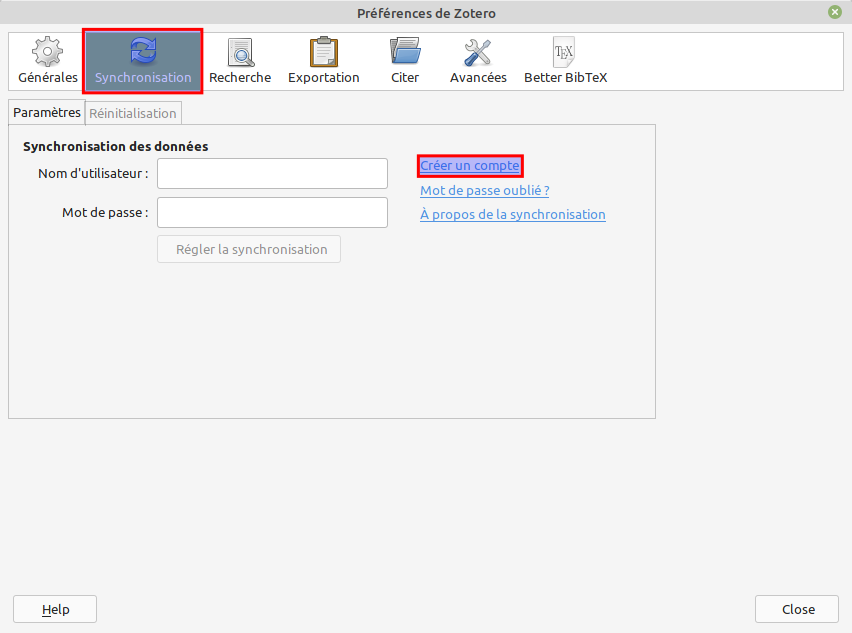
\includegraphics[width=12cm]{captures/zotero_01_compte}
					\caption{}
					\label{fig:zotero_01_compte}
				\end{figure}
			\end{center}
			\item Dans l'onglet Exportation \\
				Pour permettre le glisser-déposer de citations entre Zotero et TexStudio, choisir le format d'exportation \incmd{Better BibTeX Quick Copy}
				\begin{center}
					\begin{figure}[H]
						\centering
						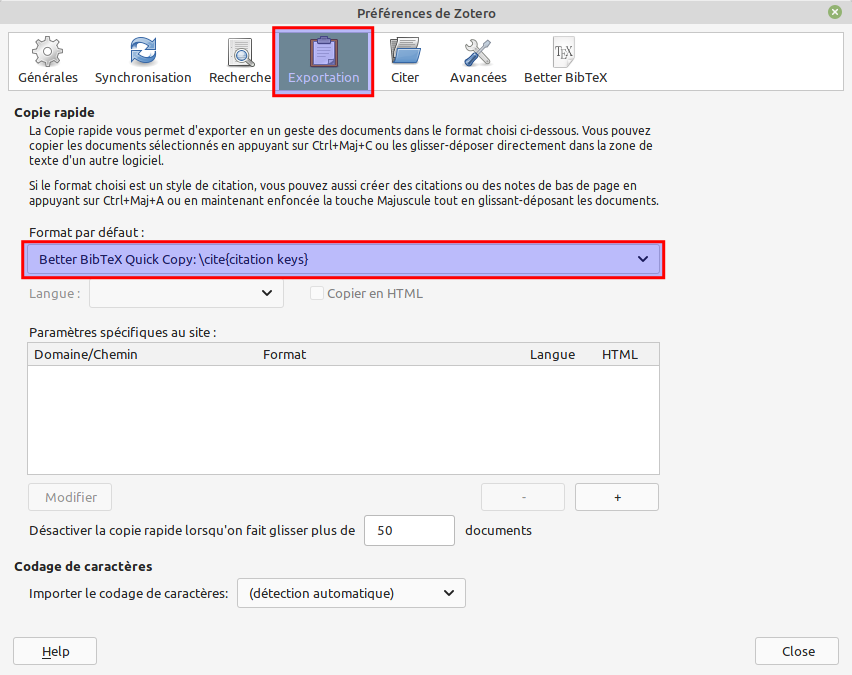
\includegraphics[width=12cm]{captures/zotero_02_exportation}
						\caption{}
						\label{fig:zotero_02_exportation}
					\end{figure}
				\end{center}
		\end{itemize}
	\item Configurer Better BibTeX.Tout se passe dans la boîte de dialogue 
			\begin{center}
				Édition \textrightarrow \ Préférences \ \textrightarrow \ Better BibTeX \textrightarrow Exportation \textrightarrow \ Copie rapide
			\end{center}
			Pour permettre le glisser-déposer de citations entre Zotero et TeXstudio, choisir le format citation LaTeX et taper autocite comme commande LaTeX.
			\begin{center}
				\begin{figure}[H]
					\centering
					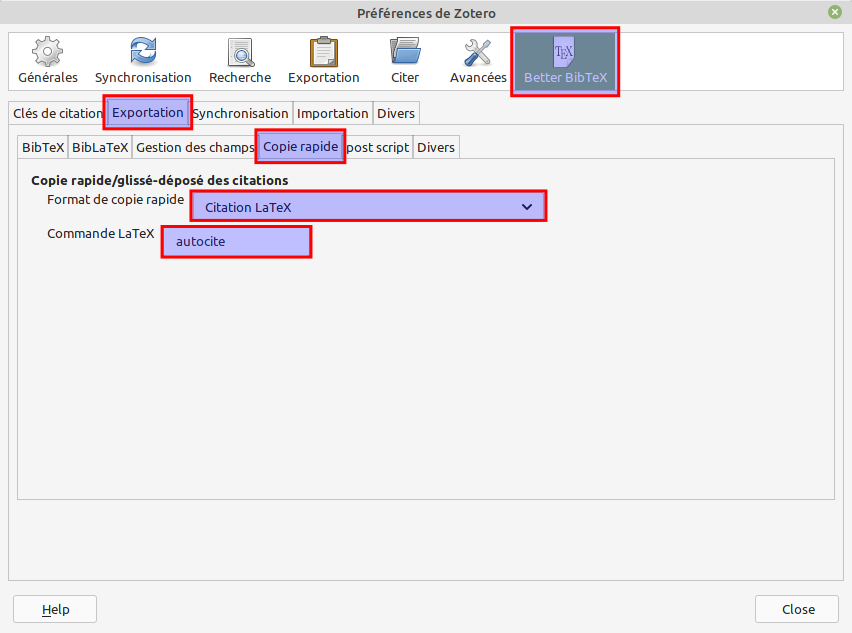
\includegraphics[width=12cm]{captures/zotero_03_better_bib_tex}
					\caption{}
					\label{fig:zotero_03_better_bib_tex}
				\end{figure}
			\end{center}
\end{enumerate}



\subsection{Configurer Texstudio}

Vérifiez que \incmd{biber} et le \incmd{Outil de bibliographie par défaut} (voir fig. \ref{fig:captureConfigBiber}).

\begin{center}
	\begin{figure}[H]
		\centering
		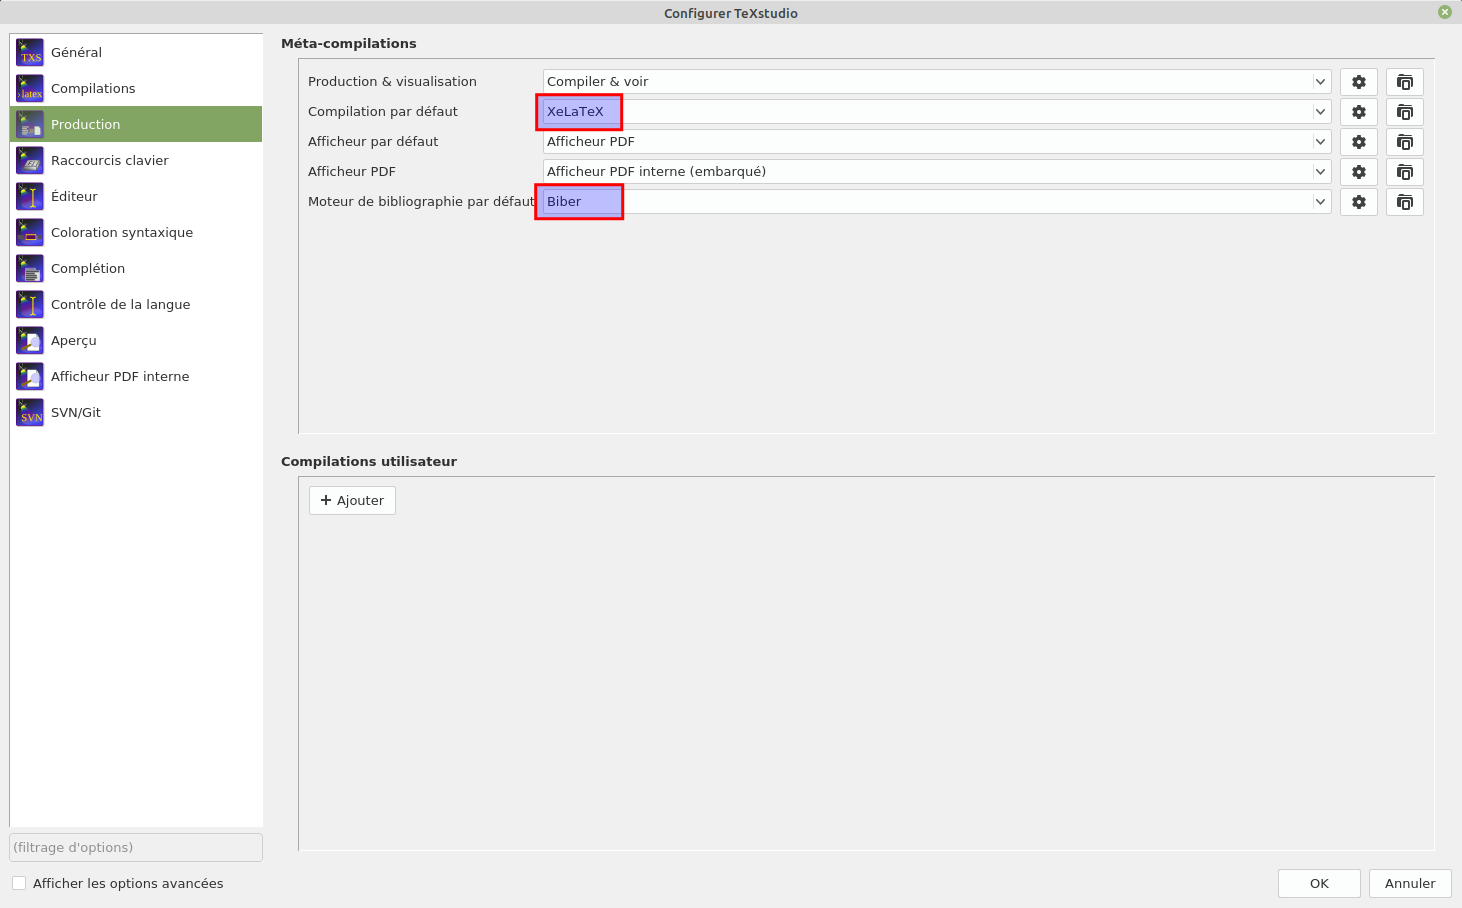
\includegraphics[width=12cm]{captures/Configurer_TeXstudio_production}
		\caption{}
		\label{fig:captureConfigBiber}
	\end{figure}
\end{center}

\nocite{CTANPackageBibLaTeX}
\printbibliography[heading=subbibliography, title=Liste des références]




\section{Index}

Pour générer un index :

\begin{enumerate}
	\item inclure un \mintinline{latex}{\makeindex} dans le préambule (ou le dé-commenter dans le template);
	\item déclarer les entrées d'index avec \mintinline{latex}{\index{entrée}};
	\item pour des sous-entrées : \mintinline{latex}{\index{Point(s)!confondus}}\mintinline{latex}{\index{Confondu(e)s!points}};
	\item placer un \mintinline{latex}{\printindex} à l'endroit où l'on veut faire afficher l'index.
\end{enumerate}

\remarque*{
	Si on veut faire des entrées d'index systématiquement pour toutes les définitions, on peut mettre \mintinline{latex}{\index} dans la définition de \mintinline{latex}{\emphdef} :
	\begin{center}
		\mintinline{latex}{\renewcommand{\emphdef}[1]{\emph{#1}\index{#1}}}.
	\end{center}
}





\end{document}
